\documentclass[11pt,a4paper,fontset=none]{ctexart}
\usepackage[margin=20mm,headheight=15pt,headsep=7mm,footskip=10mm]{geometry}
\usepackage{fontspec,xeCJK,graphicx,xcolor,booktabs,tabularx,array,enumitem,fancyhdr,hyperref,lastpage,caption,fvextra,tikz,amsmath}
\setmainfont{TeX Gyre Pagella}
\setsansfont{TeX Gyre Heros}
\setmonofont{DejaVu Sans Mono}[Scale=0.85]
\setCJKmainfont{NotoSerifCJK-Regular.ttc}[Path=/usr/share/fonts/opentype/noto/,FontIndex=3,BoldFont=NotoSerifCJK-Bold.ttc,BoldFeatures={FontIndex=3}]
\setCJKsansfont{NotoSansCJK-Regular.ttc}[Path=/usr/share/fonts/opentype/noto/,FontIndex=3,BoldFont=NotoSansCJK-Bold.ttc,BoldFeatures={FontIndex=3}]
\setCJKmonofont{NotoSansCJK-Regular.ttc}[Path=/usr/share/fonts/opentype/noto/,FontIndex=3,BoldFont=NotoSansCJK-Bold.ttc,BoldFeatures={FontIndex=3}]
\definecolor{navy}{HTML}{152F48}\definecolor{teal}{HTML}{007D86}\definecolor{ink}{HTML}{24364B}\definecolor{light}{HTML}{EAF3F4}
\pdfstringdefDisableCommands{\def\quad{ }}\color{ink}\hypersetup{colorlinks=true,linkcolor=teal,urlcolor=teal,pdftitle={PrePoMax-RCM 複材疊層設定教學},pdfauthor={Isisam},pdfsubject={RC1g2 / ccx\_fat v1.1b / v2 3D tutorial}}
\pagestyle{fancy}\fancyhf{}\fancyhead[L]{\sffamily\scriptsize PREPOMAX-RCM / 複材疊層設定教學 / RC1g2}\fancyhead[R]{\sffamily\scriptsize 2026-10-19}
\fancyfoot[L]{\sffamily\scriptsize PrePoMax-RCM\quad |\quad 作者：Isisam}\fancyfoot[R]{\sffamily\small\thepage\ /\ \pageref{LastPage}}
\renewcommand{\headrulewidth}{0.4pt}\renewcommand{\footrulewidth}{0pt}
\ctexset{section={format=\Large\sffamily\bfseries\color{navy},beforeskip=0pt,afterskip=12pt},subsection={format=\large\sffamily\bfseries\color{teal},beforeskip=9pt,afterskip=5pt}}
\urlstyle{same}\emergencystretch=3em\setlength{\parindent}{0pt}\setlength{\parskip}{6pt}\linespread{1.19}
\setlist{nosep,leftmargin=1.7em,itemsep=4pt,topsep=5pt}
\captionsetup{hypcap=false,font=small,labelfont=bf,justification=raggedright,singlelinecheck=false,skip=5pt}
\renewcommand{\arraystretch}{1.35}\newcolumntype{P}[1]{>{\raggedright\arraybackslash}p{#1}}\newcolumntype{Y}{>{\raggedright\arraybackslash}X}
\newcommand{\page}[1]{\clearpage\section*{#1}\addcontentsline{toc}{section}{#1}}
\newcommand{\cjkpath}[1]{{\small\sffamily\detokenize{#1}}}\newcommand{\key}[1]{\textsf{\textbf{#1}}}
\newcommand{\note}[1]{\par\smallskip\noindent\colorbox{light}{\parbox{\dimexpr\linewidth-2\fboxsep\relax}{\textbf{檢核重點}\quad #1}}\par\smallskip}
\newcommand{\shot}[4]{\begin{center}\par\includegraphics[width=#2\linewidth]{figs/#1}\captionof{figure}{#3}\label{#4}\end{center}}
\newcommand{\codefile}[1]{\VerbatimInput[fontsize=\small,breaklines=true,breakanywhere=true,frame=single,rulecolor=\color{teal},framesep=6pt]{evidence/#1.inp}}
\begin{document}
\renewcommand{\figurename}{圖}
{\sffamily\color{teal}\large STUDENT TUTORIAL / V2 / 3D}\par\vspace{9mm}
{\sffamily\bfseries\color{navy}\Huge PrePoMax-RCM\\[4mm]複材疊層設定教學}\par\vspace{6mm}
{\Large 用 3D 鋪層方向與俯視圖看懂角度}\par
\textbf{適用版本：RC1g2；求解器：ccx\_fat v1.1b}\par
2026 年 10 月 19 日\quad /\quad 繁體中文（台灣）\quad /\quad A4\par
\vspace{5mm}
本教學供具基本有限元素知識的碩士生獨立操作，也提供逐項證據供人工或 AI 複核。內容對應 v3 影片的 001--053 步，另補足容差、表格操作、不對稱範例與名詞對照；不需先觀看影片。
\subsection*{完成後應能做到}
\begin{enumerate}
\item 將材料、層厚與局部纖維角度指派給指定區域。
\item 區分「疊層軸」、「角度基準」與「對稱」三種設定。
\item 用 3D 預覽、俯視圖、逐層高亮、側視與實際 \texttt{.inp} 關鍵字確認設定。
\item 辨認層界不合網格、重複指派及誤用對稱等錯誤。
\end{enumerate}
\subsection*{閱讀路線}
\par\noindent\begin{tabularx}{\linewidth}{@{}lY@{}}\toprule
頁次 & 內容 \\\midrule
2--4 & 功能、角度判讀與操作前準備 \\
5--11 & 建立區域、逐層輸入、表格工具、不對稱與對稱 \\
12--14 & 每層高亮、側視與儲存前檢核 \\
15--19 & 元素集、方向、截面與求解結果 \\
20--21 & 常見錯誤、RC1g2 繁中術語 \\
22--23 & 版本、檔案位置、來源與 v3 步驟對照 \\\bottomrule
\end{tabularx}\par
\note{「對稱」是選用設定，預設為「否」。軟體可輸入任意不對稱疊層；對稱並非使用此功能的必要條件。}
\page{1\quad 功能與角度基準}
本功能（Mode A）對\textbf{既有、相容的平板三維實體網格}建立疊層：依厚度方向把區域內的元素歸入各層，並為各層建立材料、纖維方向及實體截面指派。適合已有分層網格、需要逐層指定局部角度的複材試片。
它不擠出新元素、不切割或修補元素，也不自動插入內聚力界面。研究分層或裂紋時，界面網格與疲勞內聚力模型（FATCZM）材料需另外建模。
\subsection*{三個設定要分開理解}
\par\noindent\begin{tabularx}{\linewidth}{@{}lY@{}}\toprule
設定 & 作用 \\\midrule
區域 & 決定哪些實體元素接受疊層指派，可用零件、元素集或保留的選取範圍。 \\
參考座標系（CSYS） & 定義零度纖維方向與正方向基準。使用 Global 或有效的直角座標系；材料方向 1 為纖維方向。 \\
疊層軸（1/2/3） & 參考座標系中的厚度軸。由區域節點在此軸的最小投影位置開始，沿正軸由下往上堆疊。 \\\bottomrule
\end{tabularx}\par
\subsection*{正角度遵循正疊層軸的右手定則}
\par\noindent\begin{tabularx}{\linewidth}{@{}cccY@{}}\toprule
疊層軸 & 零度纖維 & 平面第二軸 & 本地正角度方向 \\\midrule
CS 1 & CS 2 & CS 3 & CS 2 朝 CS 3 旋轉 \\
CS 2 & CS 3 & CS 1 & CS 3 朝 CS 1 旋轉 \\
CS 3 & CS 1 & CS 2 & CS 1 朝 CS 2 旋轉 \\\bottomrule
\end{tabularx}\par
若零度方向為 $\mathbf f$、平面第二軸為 $\mathbf g$，纖維方向為
\[\mathbf d_1=\cos\theta\,\mathbf f+\sin\theta\,\mathbf g.\]
本例 Rect 與全域方向一致，疊層軸為 3，因此厚度沿 $+Z$，$0^\circ$ 為 $+X$、$+90^\circ$ 為 $+Y$；$+30^\circ$ 纖維有正 $Y$ 分量。旋轉參考座標系會改變角度基準；平移只改變投影原點，不改變纖維方向。
\note{「由下往上」是沿所選正疊層軸，與螢幕目前朝向無關。示意圖的色帶有最小可見高度，不能當作精確厚度尺。}
{\small 六種方向與俯視圖見下一頁「角度判讀」。\par 技術依據：\texttt{COMPOSITE\_LAYUP.md} 的 Angle convention、Expansion and validation。}
\page{角度判讀\quad 先看基準，再看纖維}\label{pg:angles}
本頁六格均為 \textbf{RC1g2 原生 3D 面板裁切}：$0/45/90/-45$ 取自對稱例，$\pm30$ 取自兩層例。紅色板片是當次選取層；白色平行線是其纖維方向。
\begin{center}
\begin{tabular}{@{}ccc@{}}
\begin{minipage}{.31\linewidth}\centering\textbf{$0^\circ$ / P04}\par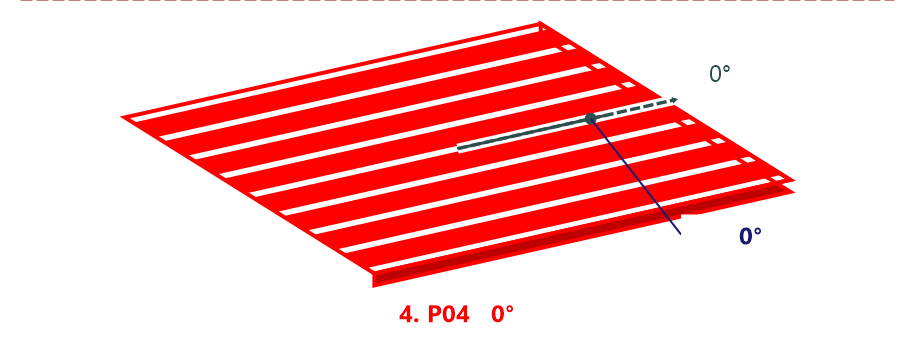
\includegraphics[width=\linewidth]{figs/sym_P04_plate.png}\par\small 與零度箭頭平行\end{minipage}&
\begin{minipage}{.31\linewidth}\centering\textbf{$+45^\circ$ / P01}\par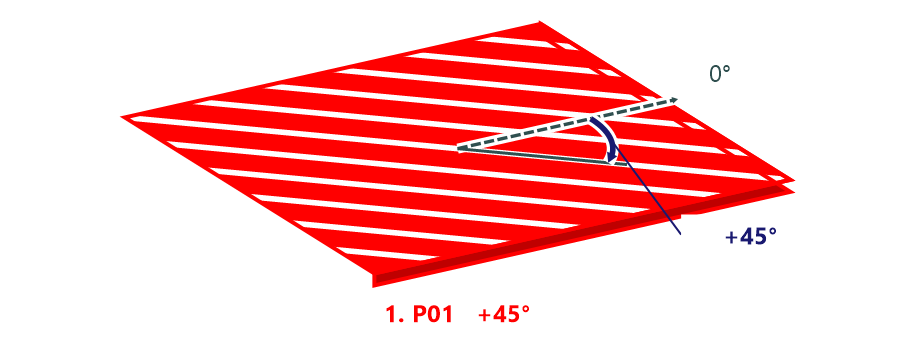
\includegraphics[width=\linewidth]{figs/sym_P01_plate.png}\par\small 從 $+X$ 朝 $+Y$ 旋轉\end{minipage}&
\begin{minipage}{.31\linewidth}\centering\textbf{$90^\circ$ / P02}\par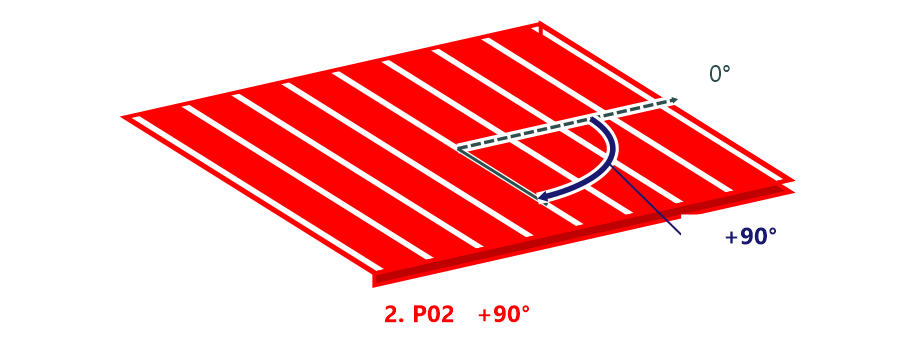
\includegraphics[width=\linewidth]{figs/sym_P02_plate.png}\par\small 與零度方向垂直\end{minipage}\\[16mm]
\begin{minipage}{.31\linewidth}\centering\textbf{$-45^\circ$ / P03}\par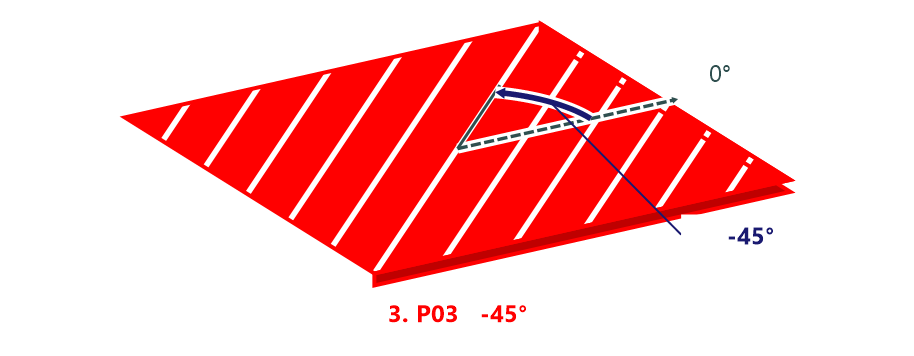
\includegraphics[width=\linewidth]{figs/sym_P03_plate.png}\par\small 從 $+X$ 朝 $-Y$ 旋轉\end{minipage}&
\begin{minipage}{.31\linewidth}\centering\textbf{$+30^\circ$ / P01}\par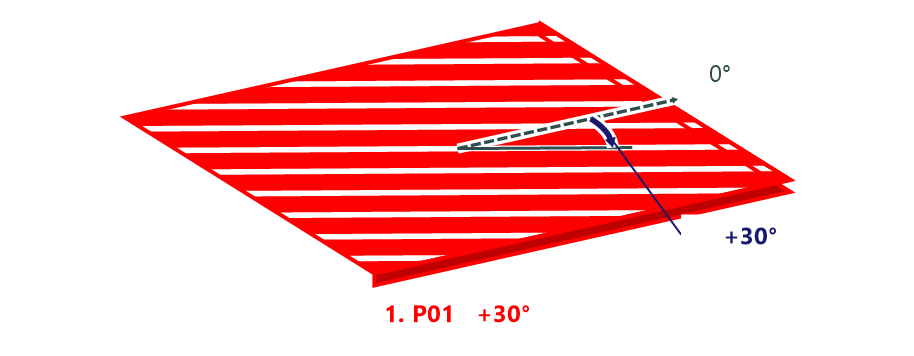
\includegraphics[width=\linewidth]{figs/two_P01_plate.png}\par\small 正角度，纖維朝 $+Y$\end{minipage}&
\begin{minipage}{.31\linewidth}\centering\textbf{$-30^\circ$ / P02}\par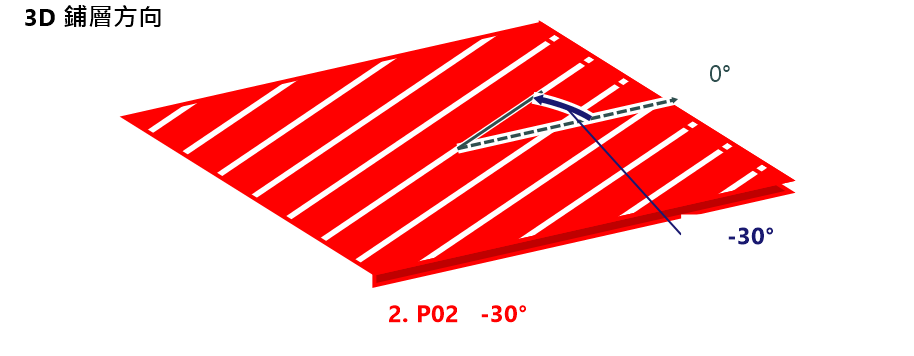
\includegraphics[width=\linewidth]{figs/two_P02_plate.png}\par\small 負角度，纖維朝 $-Y$\end{minipage}
\end{tabular}
\captionof{figure}{六種方向並排比較。斜視投影會改變螢幕上的夾角；讀原生角度弧與標值，不拿量角器量斜視圖。}\label{fig:angles}
\end{center}
\begin{center}
\begin{minipage}[t]{.48\linewidth}\centering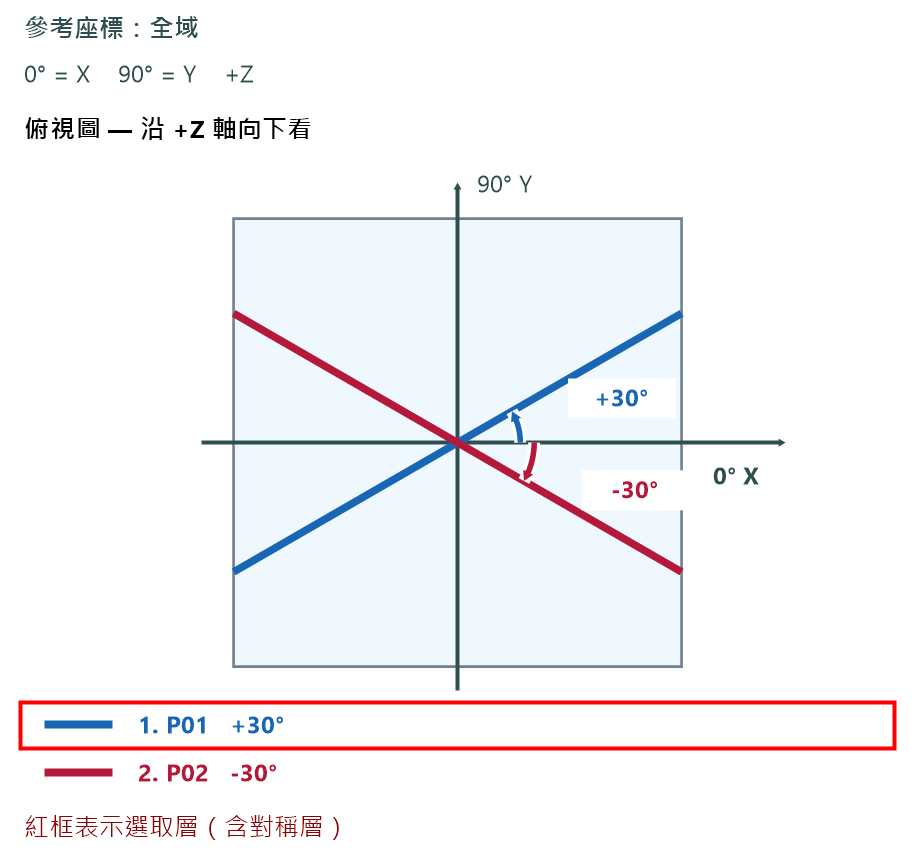
\includegraphics[height=62mm]{figs/two_P01_plan.png}\par\small 兩層：$+30/-30$ 的 X\end{minipage}\hfill
\begin{minipage}[t]{.48\linewidth}\centering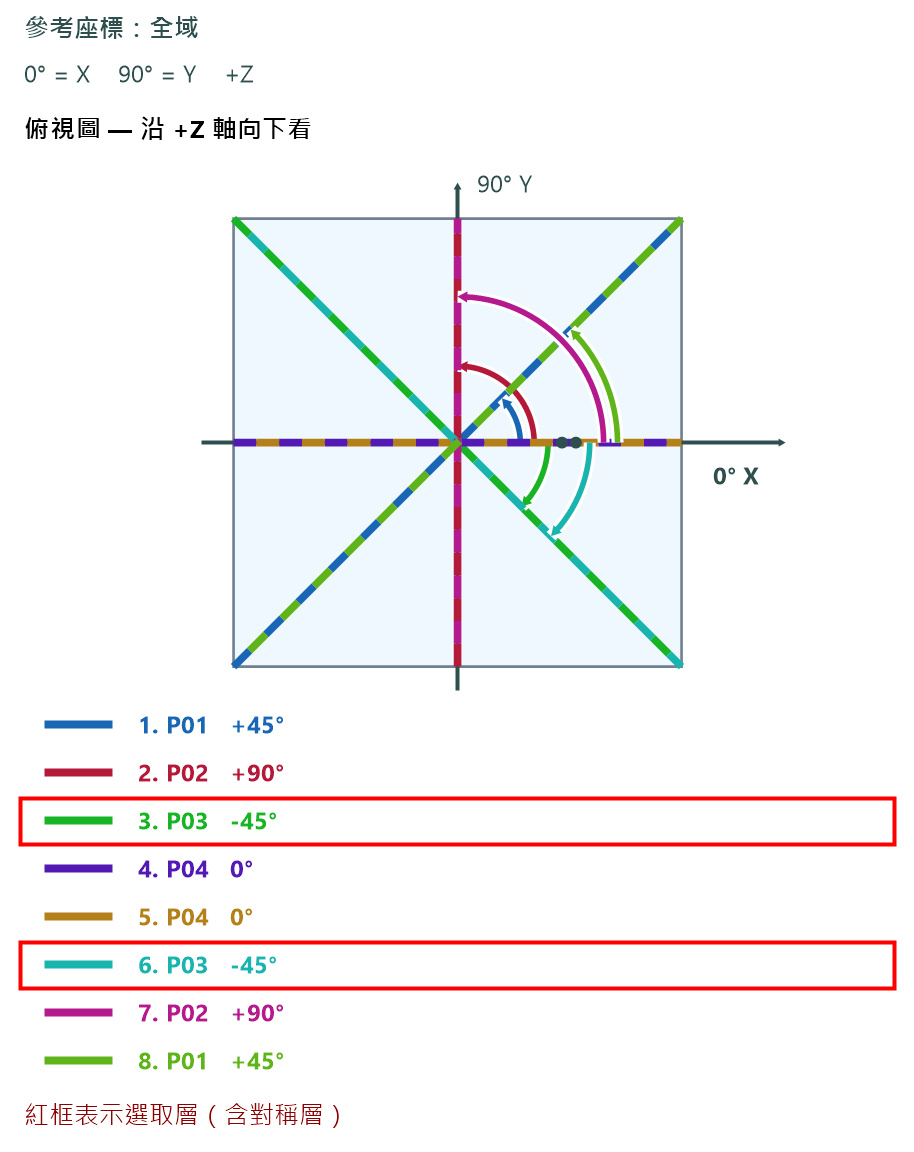
\includegraphics[height=62mm]{figs/sym_P03_plan.png}\par\small 對稱例：$\pm45$ 的 X，另有 $0/90$\end{minipage}
\captionof{figure}{RC1g2 俯視圖與完整圖例。相同角度的對稱層共線，以交替色段分辨；紅框圈出所選層及對稱夥伴。}\label{fig:plans}
\end{center}
\textbf{讀圖順序：}先找 $0^\circ$ 虛線箭頭，再沿角度弧讀正負旋轉（$0^\circ$ 為起點圓點），最後看板片的平行纖維線。本例疊層軸 3，從 $+Z$ 朝原點看，$+X$ 向右、$+Y$ 向上，正角度逆時針。俯視彩線是各層方向，\textbf{彩線本身的紅色不代表選取}；用紅框、紅板片及 P 編號判讀。
\note{3D 為分離板片示意，層間距與可見高度不是厚度尺。對稱夥伴保留原角度，不因鏡射自動變號；對稱可選，預設「否」。}

\page{2\quad 操作前準備}
\begin{enumerate}
\item 使用已完整解壓縮的 \textbf{PrePoMax-RCM RC1g2}。發行檔為\par
\texttt{PrePoMax-RCM\_win64\_RC1g2.zip}。\par
開啟解壓後的 \texttt{PrePoMax.exe}，保留相鄰的 \texttt{Solver}、\texttt{lib} 等資料夾。解壓後可直接執行。
\item 若需切換語言：\key{工具 → 設定 → 一般 → 語言 → 繁體中文}。切換後以實際欄位內容對照本文第 21 頁術語表。
\item 建立自己的可寫入工作資料夾，例如自行建立的 LayupPractice 資料夾。將本教學 \texttt{examples/} 內的檔案複製到該資料夾；不要直接修改來源。
\item 選\key{檔案 → 開啟}讀取 \texttt{coupon\_no\_layup.inp}。匯入時確認\textbf{三維實體（3D）、長度 mm}；模型使用 N、mm、MPa。另存為自己的 \texttt{Walkthrough\_student.pmx}。
\end{enumerate}
\subsection*{本例的起點與基準檔}
\par\noindent\begin{tabularx}{\linewidth}{@{}lY@{}}\toprule
檔案／項目 & 用途與預期 \\\midrule
\texttt{coupon\_no\_layup.inp} & 無疊層起點：4 × 2 × 1 mm，64 個 C3D8I，厚度方向 8 層，每層 0.125 mm。保留材料及靜態邊界條件。 \\
自行儲存的 \texttt{.pmx} & 依第 5--14 頁建立疊層後儲存，作為自己的可編輯基準；本來源包不附完成的 PMX。 \\
\texttt{walkthrough\_export.inp} & 已完成的扁平化求解輸入，用於核對關鍵字。 \\
發行包 \texttt{Examples/Layup/} & 有 \texttt{Layup.pmx}、\texttt{Layup.inp} 等範例；其中 \texttt{.inp} 已含展開後指派，不可直接再疊加本教學的新指派。 \\
\texttt{IM7\_8552} & 起點內已有的正交異向性材料；本教學所有層均使用此實際名稱。 \\\bottomrule
\end{tabularx}\par
\note{先檢查材料、零件與網格存在。匯入 \texttt{.inp} 不會無損還原可編輯的疊層物件；要保留疊層編輯能力，必須儲存 \texttt{.pmx}。}
\subsection*{截圖的版本與閱讀方式}
新增的 3D 鋪層方向與俯視圖均由 RC1g2 原生編輯器重新擷取，只保留面板內容。舊表單／VTK 圖仍來自 RC1c 的 v3 操作影格，圖說分別標示來源；既有求解數值沿用 RC1f/v1.1b 證據。本次未另跑 FEM；RC1g2 套件的獨立驗收與本教學的圖文檢查範圍分開。
\page{3\quad 建立疊層並指定區域}
\textbf{操作 01（v3 001--005）}
\begin{enumerate}
\item 在\key{模型（Model）}樹的\key{複材疊層（Composite Layups）}上按右鍵，選\key{建立（Create）}。之後可雙擊物件重新編輯。
\item 名稱輸入 \texttt{Walkthrough}。區域類型選\key{零件名稱（Part name）}，再選 \texttt{Solid\_part-1}（見圖\ref{fig:region}）。
\item 若模型名稱不同，選包含整個試片、64 個元素的實體零件；不要選到節點集、殼或界面材料區。
\end{enumerate}
\shot{s005_form.png}{0.94}{指定整個試片零件。來源：v3 步驟 005 原生編輯器；此時尚未完成逐層輸入。}{fig:region}
\textbf{其他區域方式：}若只對部分元素疊層，可選\key{元素集名稱（Element set name）}並指定既有元素集；或選\key{選取（Selection）}並選取目標實體元素。以元素高亮確認完整範圍，避免遺漏或誤選其他零件。
\note{一個區域不可同時由兩個啟用的疊層，或由疊層與一般材料截面重複覆蓋。若以已完成範例練習，先在副本停用舊疊層／移除衝突指派。}
\page{4\quad 參考座標系、疊層軸與容差}
\textbf{操作 02（v3 006--007）}
\begin{enumerate}
\item \key{座標系統}選 \texttt{Rect}，\key{疊層軸}選 \texttt{3}。本例 Rect 的三軸分別對齊全域 X、Y、Z；若沒有此項，可選\key{Global／全域}，本例方向相同。
\item \key{對稱}先保留\key{否}。四列輸入完成後，才在第 11 頁切為\key{是}。
\item \key{邊界容差}保留 \texttt{1E-06}（圖\ref{fig:axis}）。它是\textbf{相對值}，不是 mm。
\end{enumerate}
\begin{center}\par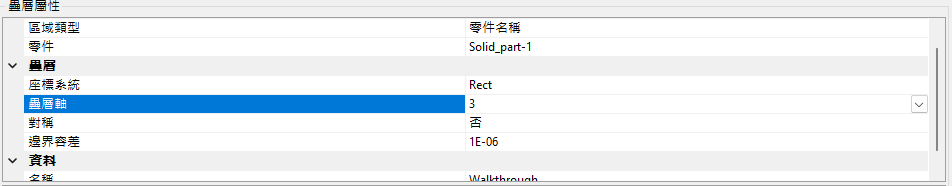
\includegraphics[width=\linewidth]{figs/axis_detail.png}\captionof{figure}{座標系、疊層軸、對稱與邊界容差。由步驟 007 的原生表單裁切，未改動欄位內容。}\label{fig:axis}\end{center}
\subsection*{容差的量級}
完整展開厚度為 $H$ 時，絕對容差為
\[\delta=H\times\text{BoundaryTolerance}.\]
本例完成後 $H=1$ mm，所以 $\delta=10^{-6}$ mm。區域在疊層軸的節點投影厚度，必須與 $H$ 一致；每個元素的全部節點（含中間節點）也必須落在同一層區間內。
\subsection*{先核對方向再填角度}
在全域／Rect 第三軸設定下，由 $z=0$ 開始往 $z=1$ mm 排列。若試片厚度沿別的方向，先選正確座標系與軸；不要只調整角度來掩蓋厚度方向選錯。
\note{容差須為有限值且 $0\leq\text{容差}<0.5$。保留預設值；若元素跨層，修正網格或層厚，不要放大容差讓錯誤消失。}
{\small 本頁的容差說明補充影片 007；依據 \texttt{COMPOSITE\_LAYUP.md}。}
\begin{center}
\begin{minipage}{.30\linewidth}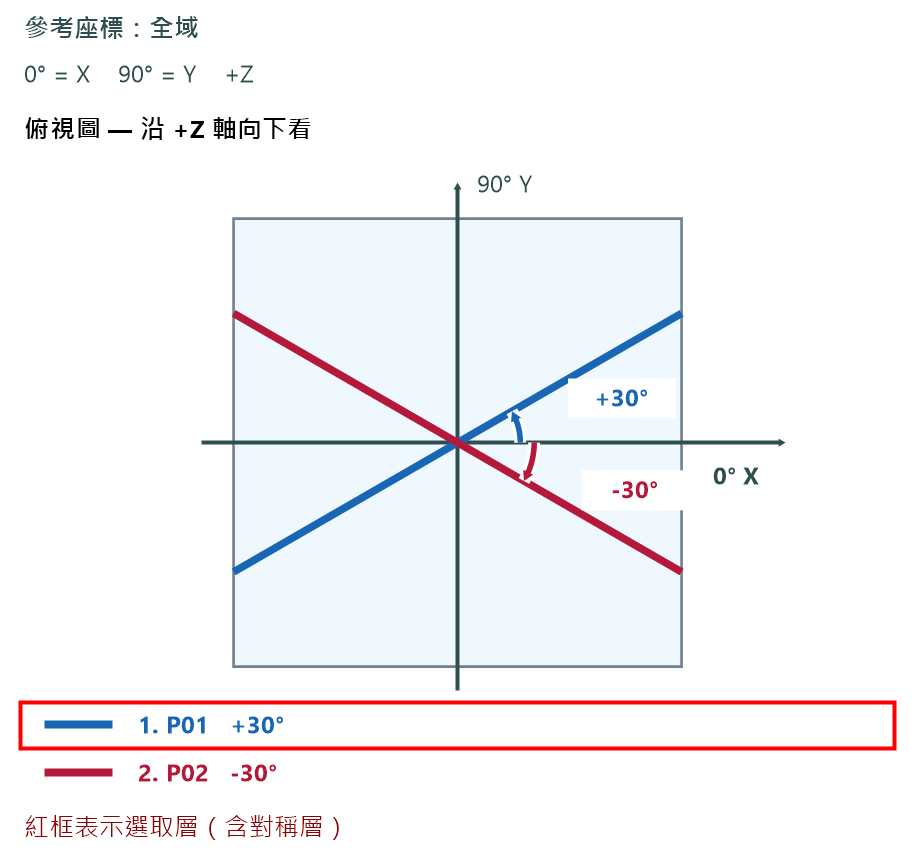
\includegraphics[width=\linewidth]{figs/two_P01_plan.png}\end{minipage}\hfill
\begin{minipage}{.64\linewidth}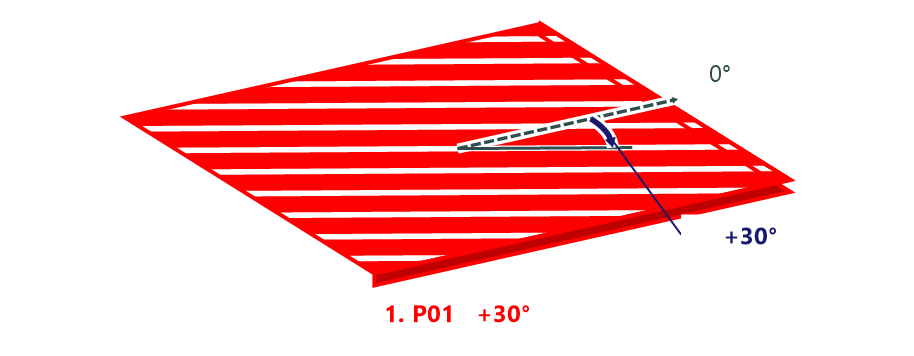
\includegraphics[width=\linewidth]{figs/two_P01_plate.png}\end{minipage}
\captionof{figure}{RC1g2 全域／軸 3 的讀圖範例：俯視的 $0^\circ$ 箭頭為 $+X$，角度弧從此起算；右側紅板片為所選 P01（$+30^\circ$），白線為纖維。無對稱夥伴。}\label{fig:axisnative}
\end{center}

\page{5\quad 逐欄輸入第一層 P01}\label{pg:firstply}
\textbf{操作 03（v3 008--012）}
\begin{enumerate}
\item 點第一列\key{名稱}，改為 \texttt{P01}；\key{材料}下拉選 \texttt{IM7\_8552}。
\item \key{厚度}輸入 \texttt{0.125 mm}，\key{角度}輸入 \texttt{45}（度）。完成每格後按 \key{Tab} 提交，再閱讀驗證摘要。
\item \key{元素}輸入 \texttt{1}：檢查這一層是否恰有\textbf{一個既有厚度網格帶}。
\end{enumerate}
\begin{center}\par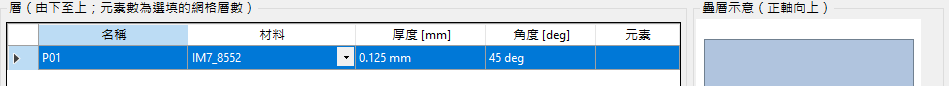
\includegraphics[width=\linewidth]{figs/ply01_detail.png}\captionof{figure}{P01 的名稱、材料、厚度與角度已填入；來源為 v3 步驟 011。此影格的「元素」仍空白，下一步 012 才填入 1。}\label{fig:ply01}\end{center}
\begin{center}
\begin{minipage}[c]{.28\linewidth}\par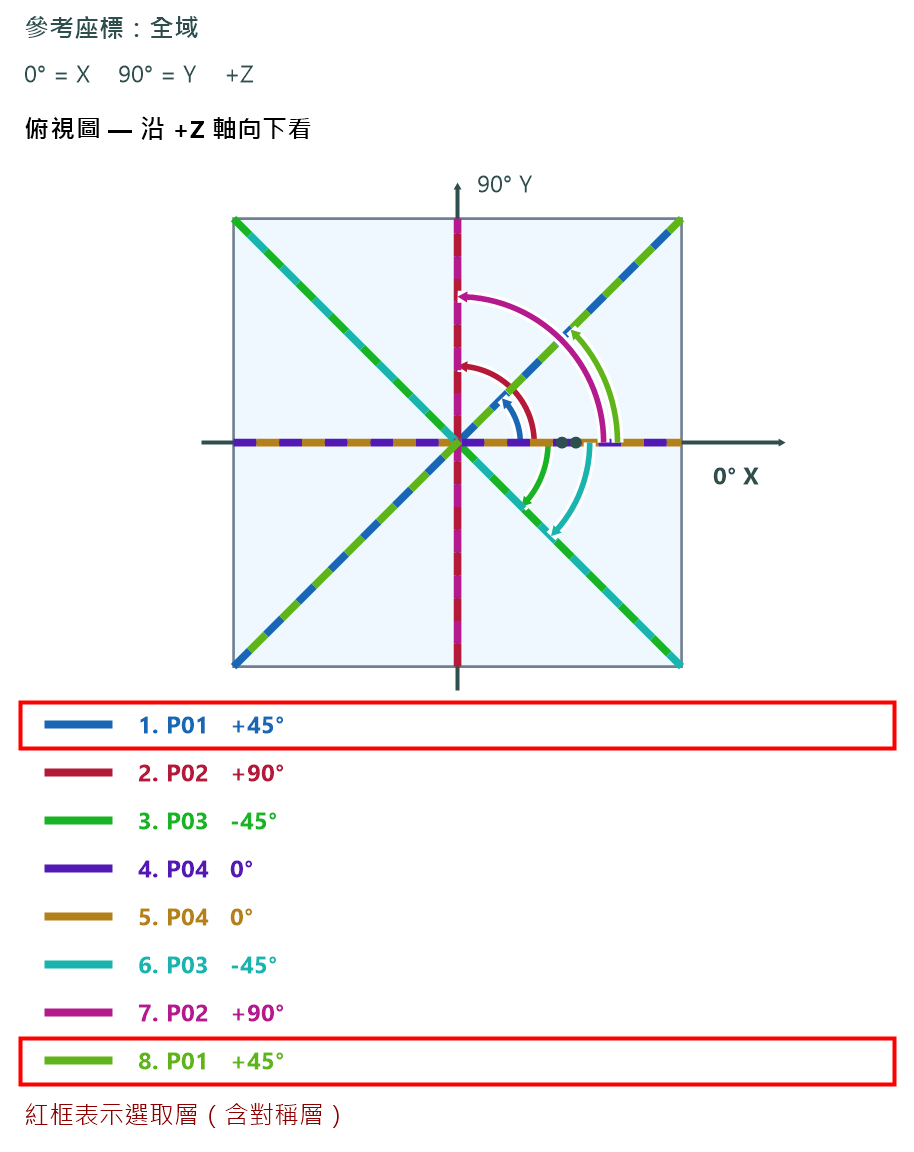
\includegraphics[width=\linewidth]{figs/sym_P01_plan.png}\end{minipage}\hfill
\begin{minipage}[c]{.68\linewidth}\par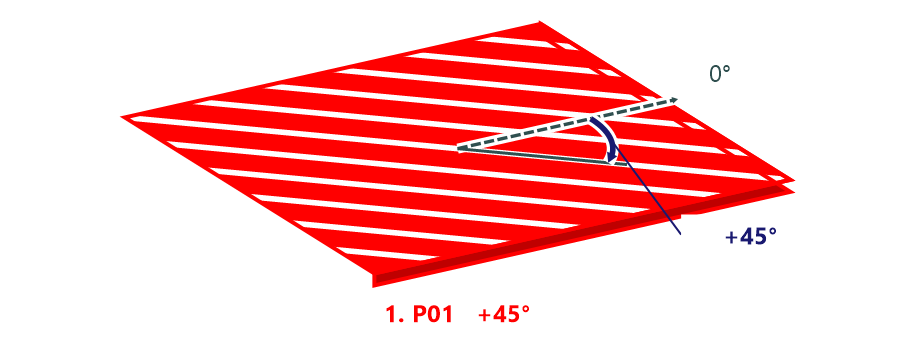
\includegraphics[width=\linewidth]{figs/sym_P01_plate.png}\end{minipage}
\captionof{figure}{RC1g2 完成例中選 P01：左為俯視圖與紅框，右為最低的 45 度紅板片。此圖為完成後的角度對照，不是只輸入第一列時的驗證狀態。}\label{fig:first3d}\end{center}
如圖\ref{fig:ply01}，表格由下往上定義實體堆疊；第一列是最低的一層。完成第一層時輸入厚度只有 0.125 mm，而區域厚度為 1 mm，因此整體檢核暫時未通過是預期狀態。
\subsection*{數值與材料的意義}
\par\noindent\begin{tabularx}{\linewidth}{@{}lY@{}}\toprule
欄位 & 填寫規則 \\\midrule
材料 & 必須存在且啟用；名稱是識別資料，不翻譯或任意改成中文。 \\
厚度 & 正的有限長度，可用目前模型單位或明寫 \texttt{0.125 mm}；須與厚度網格一致。 \\
角度 & 有限度數，可為正、負、零；正號依正疊層軸的右手定則。 \\
元素 & 選填的正整數。是厚度網格帶數，不是元素編號、元素總數，也不是網格生成命令；留空只略過帶數檢查。 \\\bottomrule
\end{tabularx}\par
\note{表達式在輸入時會換算成模型數值，不是持續連動的公式。本例一層有 8 個實體元素，但「元素」欄仍填 1。}
\page{6\quad 新增 P02、P03、P04}
\textbf{操作 04（v3 013--030）}
按\key{新增}建立下一列，逐欄輸入下表；每完成一格按 \key{Tab}。新增 P02、P03、P04 時，分別對應影片的 013、019、025 步。
\par\noindent\begin{tabularx}{\linewidth}{@{}lYrrr@{}}\toprule
名稱 & 材料 & 厚度（mm） & 角度（度） & 元素 \\\midrule
P01 & \texttt{IM7\_8552} & 0.125 & 45 & 1 \\
P02 & \texttt{IM7\_8552} & 0.125 & 90 & 1 \\
P03 & \texttt{IM7\_8552} & 0.125 & $-45$ & 1 \\
P04 & \texttt{IM7\_8552} & 0.125 & 0 & 1 \\\bottomrule
\end{tabularx}\par
\begin{center}\par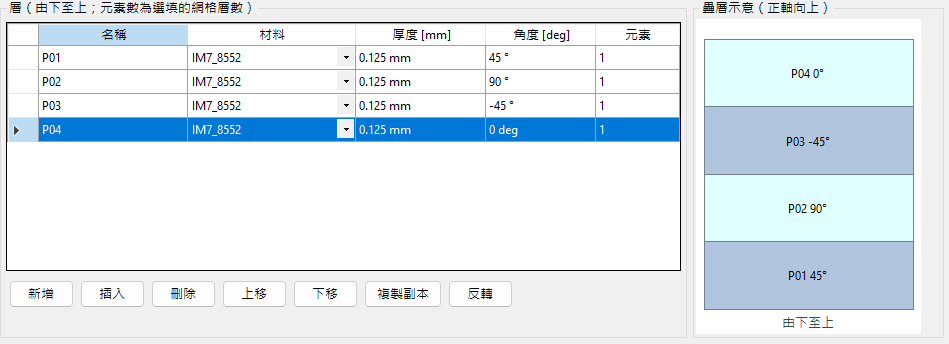
\includegraphics[width=.70\linewidth]{figs/four_plies_detail.png}\captionof{figure}{四列輸入完成，右側舊圖以色帶列出 45／90／−45／0 度；方向請另看 RC1g2 圖\ref{fig:angles}與圖\ref{fig:plans}。來源：v3 步驟 030 的表格與疊層圖。}\label{fig:four}\end{center}
用第\pageref{pg:angles}頁的 3D 纖維線及俯視 X 逐一比對四種方向：先以 $0^\circ$ 箭頭定基準，再看角度弧；紅色板片表示選取層。比較圖\ref{fig:four}與上表：P03 的負號不可漏掉；四列厚度都應為 0.125 mm。此時\key{對稱＝否}，總厚度只有 $4\times0.125=0.5$ mm，尚未覆蓋 1 mm 試片。
\note{暫時的厚度不符不代表必須使用對稱。要做四層不對稱設計，請讓各層厚度合計為 1 mm 且每個層界吻合網格；本次為重現 v3，下一步使用四列對稱展開。}
\begin{center}
\begin{minipage}{.30\linewidth}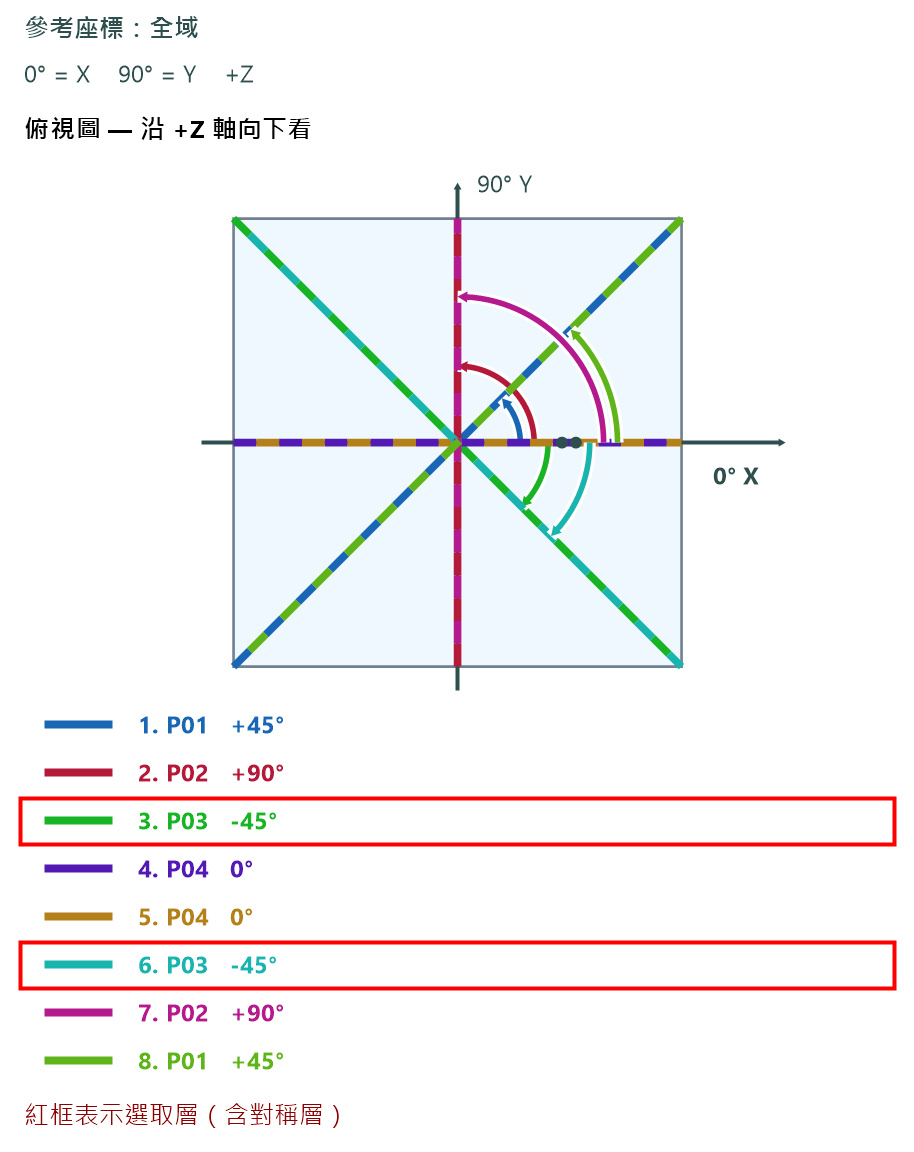
\includegraphics[width=\linewidth]{figs/sym_P03_plan.png}\end{minipage}\hfill
\begin{minipage}{.64\linewidth}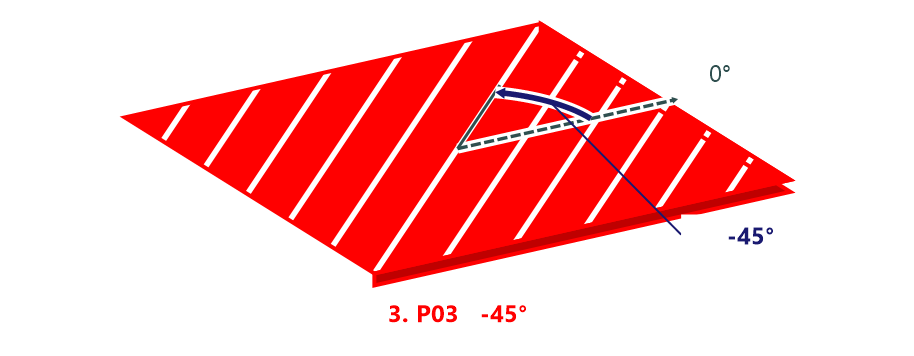
\includegraphics[width=\linewidth]{figs/sym_P03_plate.png}\end{minipage}
\captionof{figure}{RC1g2 完成例選 P03：俯視彩線同時呈現四種方向；右側 $-45^\circ$ 紅板片的角度弧與纖維線可對照零度箭頭。完成例已開對稱，紅框另圈出第 6 層夥伴；本頁輸入階段仍為「否」。}\label{fig:fournative}
\end{center}

\page{7\quad 表格工具與對稱設計觀念}
\textbf{操作 05（補充影片的表格操作）}\par 先對照圖\ref{fig:buttons}找到各個按鈕，再在副本中練習。
\begin{center}\par
\includegraphics[width=0.94\linewidth]{figs/buttons_detail.png}\captionof{figure}{表格工具列：新增、插入、刪除、上移、下移、複製副本與反轉。來源：步驟 030 原生編輯器裁切。}\label{fig:buttons}\end{center}
\par\noindent\begin{tabularx}{\linewidth}{@{}lY@{}}\toprule
操作 & 可直接練習的方式 \\\midrule
新增／插入 & 新增下一列；若要在所選列位置加層，先選該列再按插入。 \\
複製副本 & 選 P01 後按複製副本，再將新列改名、改角度。副本可獨立編輯；完成後核對列數與順序。 \\
上移／下移 & 選列後移動，會改變由下往上的實體順序；不是只改顯示排序。 \\
反轉 & 將目前輸入層清單順序顛倒；例如 45/90/−45/0 變為 0/−45/90/45。角度符號不會因此自動反號。 \\
刪除 & 刪除所選列後，重新檢查總厚度。要放棄整次編輯請用取消。 \\\bottomrule
\end{tabularx}\par
\subsection*{為什麼常用對稱？}
對稱是設計慣例：在經典層板理論的條件下，關於中面對稱的材料與層厚配置使拉伸與彎曲耦合矩陣 $B=0$，可避免此類耦合，並降低相關翹曲傾向；它不保證所有載重、邊界或溫度條件下都不翹曲。軟體也接受不對稱配置。

\page{7A\quad 兩層不對稱：看見 +30／−30}\label{pg:two}
\subsection*{兩層 $[+30/-30]$：可以輸入的不對稱疊層}
另開起點副本，建立 \texttt{Unsymmetric30}；區域、Rect／軸 3 與本例相同，\textbf{對稱保持「否」}。輸入：
\par\noindent\begin{tabularx}{\linewidth}{@{}lYrrr@{}}\toprule
名稱 & 材料 & 厚度（mm） & 角度（度） & 元素 \\\midrule
P01 & \texttt{IM7\_8552} & 0.5 & $+30$ & 4 \\
P02 & \texttt{IM7\_8552} & 0.5 & $-30$ & 4 \\\bottomrule
\end{tabularx}\par
在本教學八帶網格上，兩層各使用四個厚度帶，總厚度仍為 1 mm。選 P01 應覆蓋 $z=0$--0.5 mm，選 P02 應覆蓋 $z=0.5$--1 mm，各 32 個元素。這是可重做的設定練習，非 v3 影片中另一次已執行求解的結果。
\begin{center}
\begin{minipage}[t]{.48\linewidth}\centering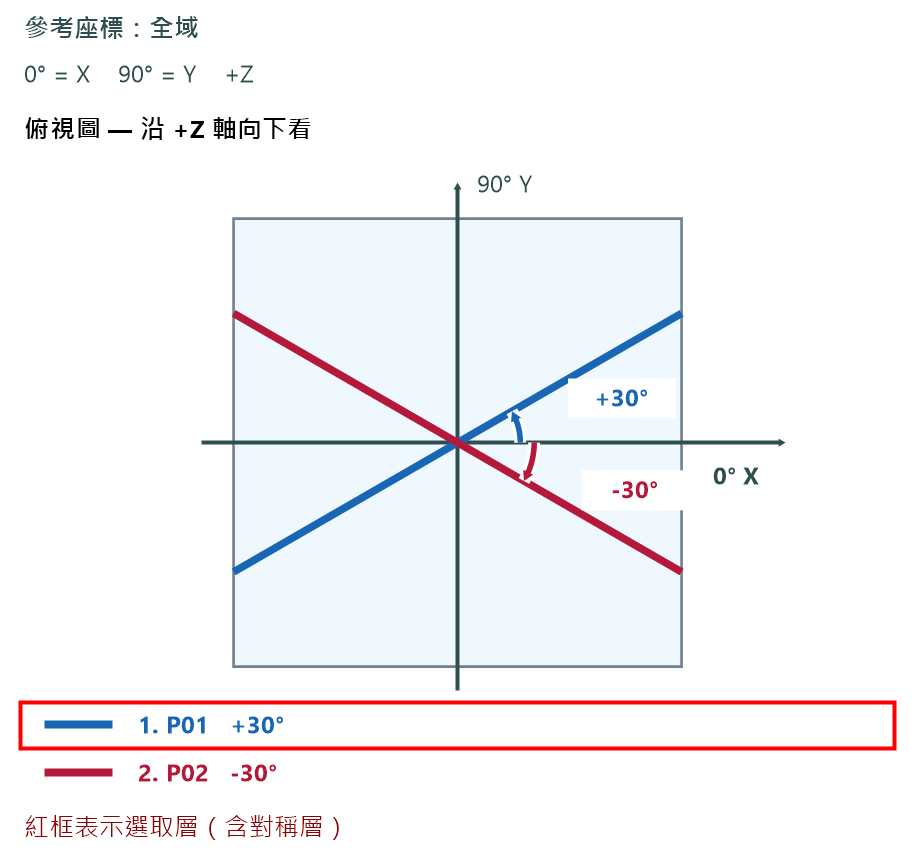
\includegraphics[width=\linewidth]{figs/two_P01_plan.png}\par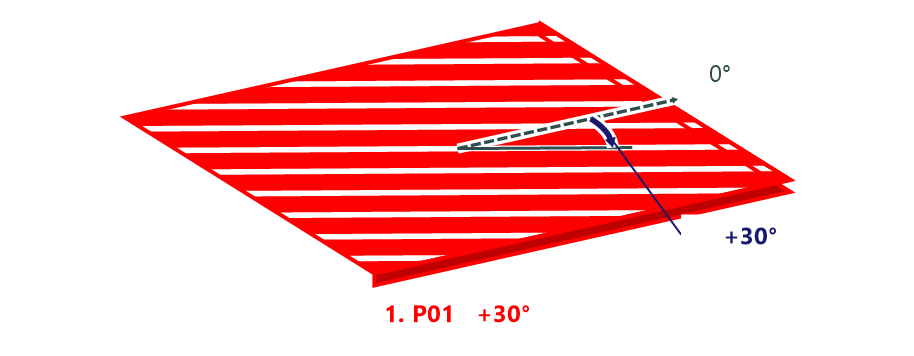
\includegraphics[width=\linewidth]{figs/two_P01_plate.png}\end{minipage}\hfill
\begin{minipage}[t]{.48\linewidth}\centering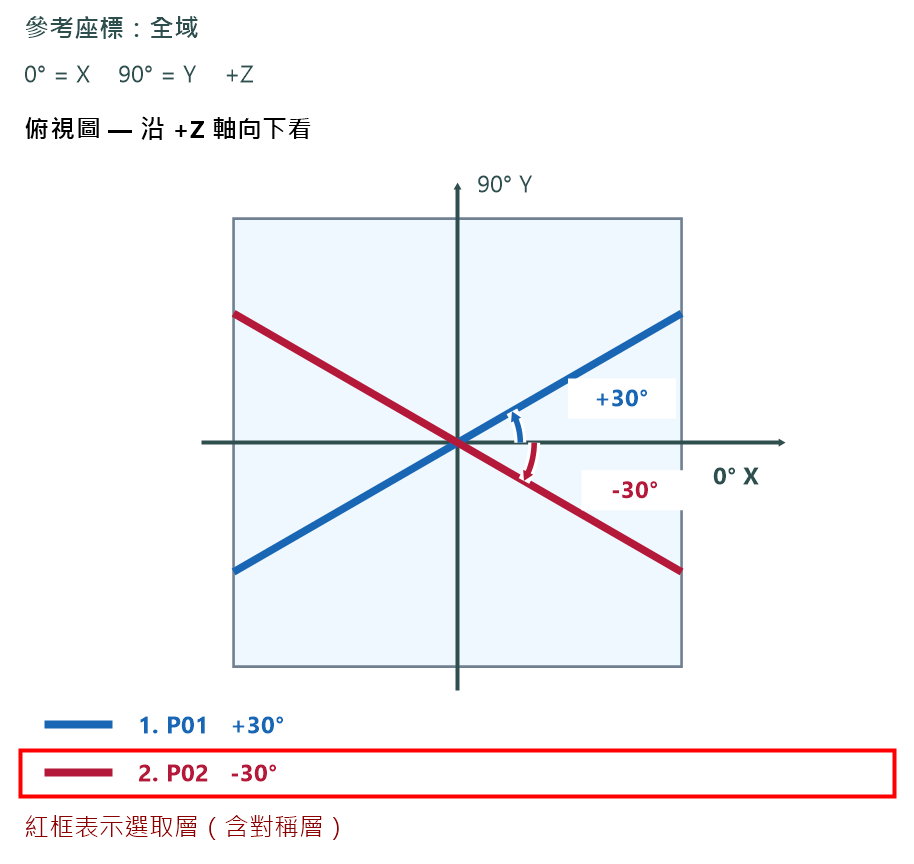
\includegraphics[width=\linewidth]{figs/two_P02_plan.png}\par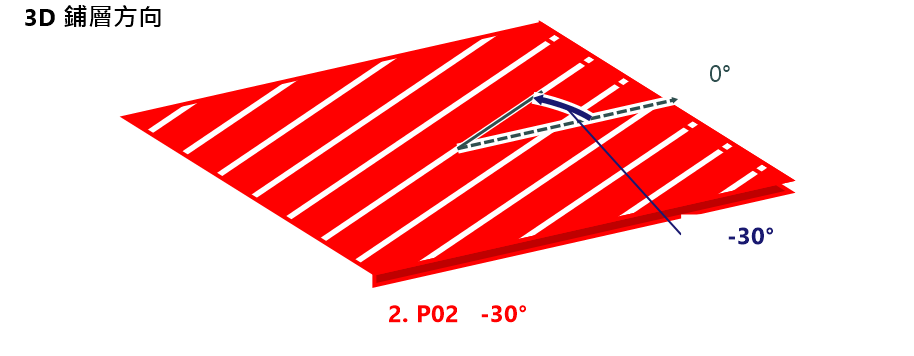
\includegraphics[width=\linewidth]{figs/two_P02_plate.png}\end{minipage}
\captionof{figure}{RC1g2：左選 P01（$+30^\circ$），右選 P02（$-30^\circ$）。兩次俯視均有 X；紅框和紅板片隨選列移動，角度及彩線不變。3D 只裁出當次所選板片。}\label{fig:two3d}
\end{center}
先找 $0^\circ$ 箭頭，沿正／負角度弧到纖維線。兩層無對稱夥伴，各自只選取一個實體層；$+30$ 與 $-30$ 不可互換。以上兩次驗證均為兩層、64 元素有效配置。

\note{$[+30/-30]$ 具有正負角度配對，但對中面不對稱；「平衡」與「對稱」不同。完成練習後取消或保留獨立檔案，不可與 Walkthrough 同時啟用覆蓋同一區域。}
\page{8\quad 選用對稱：四列展開成八層}\label{pg:sym}
\textbf{操作 06（v3 031--032）}
回到四列 \texttt{Walkthrough}，將\key{對稱}由預設\key{否}改為\key{是}。如圖\ref{fig:sym}，程式將\textbf{完整反向清單接在原清單後面}，中心層也複製：
\[ [45/90/-45/0]_s=[45,90,-45,0,0,-45,90,45]. \]
由 $+Z$ 起點到終點共八層；$H=8\times0.125=1$ mm。虛線中面在兩個 $0^\circ$ 層之間（$z=0.5$ mm），不是在其中一層中央。
\begin{center}\par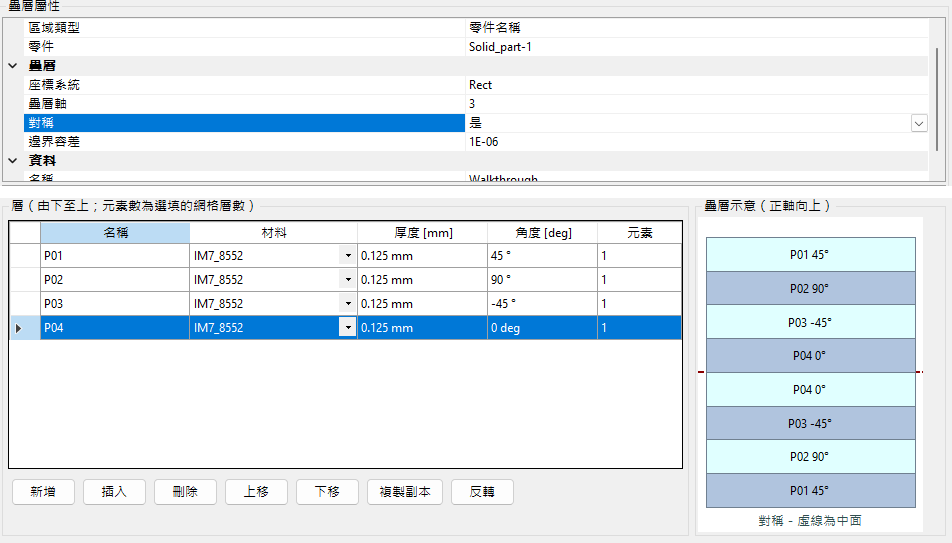
\includegraphics[width=0.60\linewidth]{figs/symmetry_detail.png}\captionof{figure}{對稱設定與八層圖：P01／P02／P03／P04／P04／P03／P02／P01。來源：v3 步驟 031 的原生編輯器。}\label{fig:sym}\end{center}
\begin{center}
\begin{minipage}[c]{.30\linewidth}\par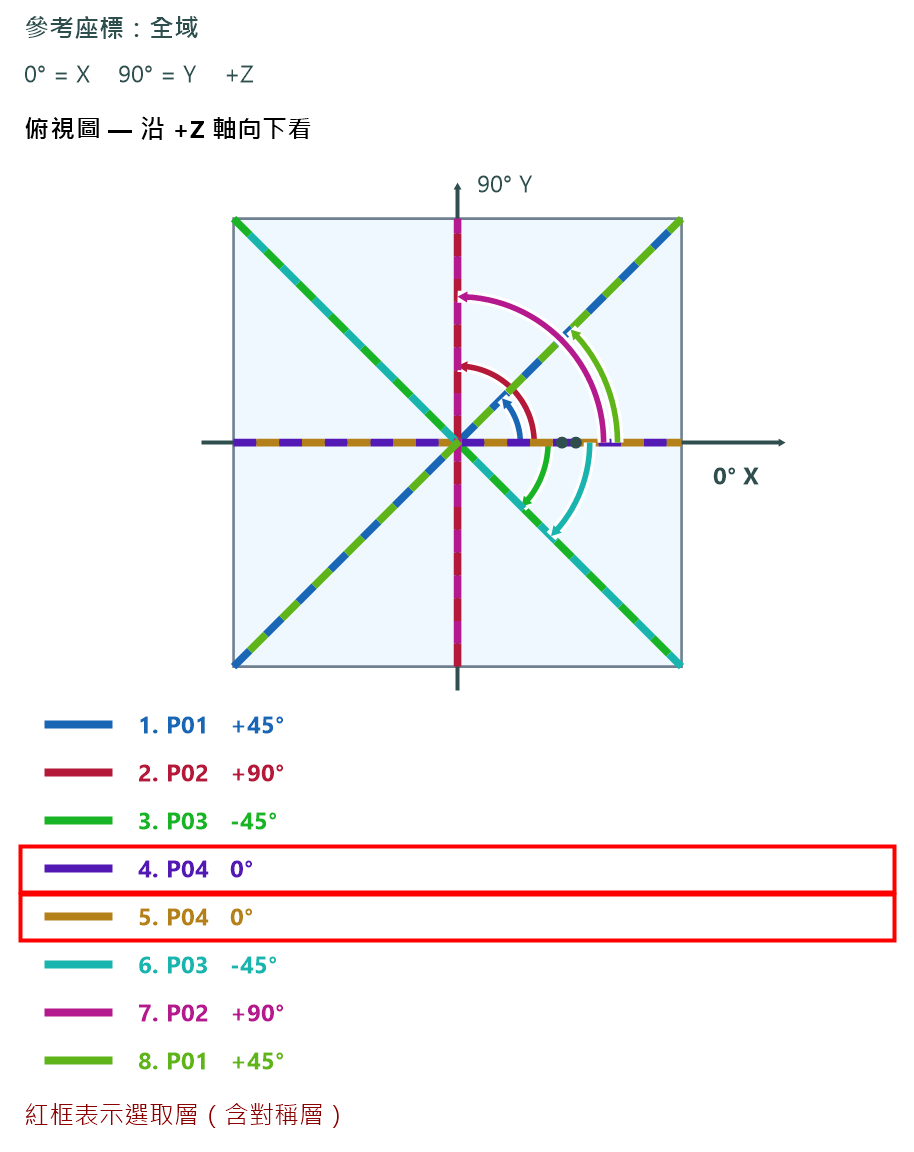
\includegraphics[width=\linewidth]{figs/sym_P04_plan.png}\end{minipage}\hfill
\begin{minipage}[c]{.65\linewidth}\par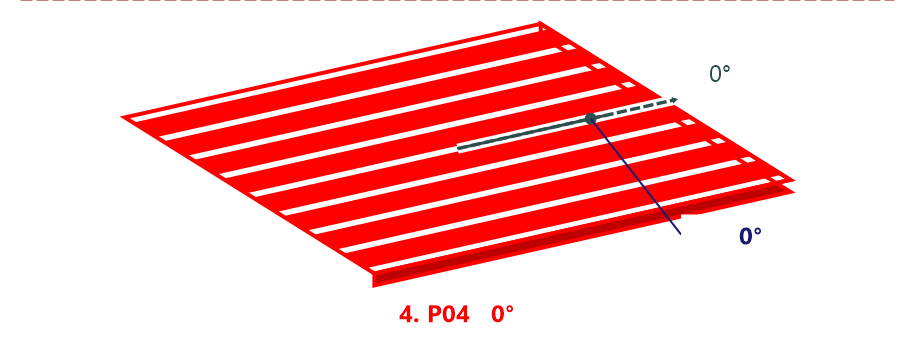
\includegraphics[width=\linewidth]{figs/sym_P04_plate.png}\end{minipage}
\captionof{figure}{RC1g2 對稱例選 P04：俯視紅框同時標示第 4、5 層；右為第 4 層的 0 度纖維與零度箭頭。}\label{fig:sym3d}\end{center}
\note{若已輸入完整八層，再選「是」會變成 16 層。本例只輸入四列；對稱後總厚度必須為 1 mm。}
\page{9\quad 逐層高亮：先看 P01}
\textbf{操作 07（v3 033--034）}
選表格 P01 一列。對稱已開啟時，兩個對應實體層都應變紅，不能只看到一端就判定正確。以滑鼠中鍵／滾輪拖曳旋轉，再從側面看厚度位置。
\begin{center}
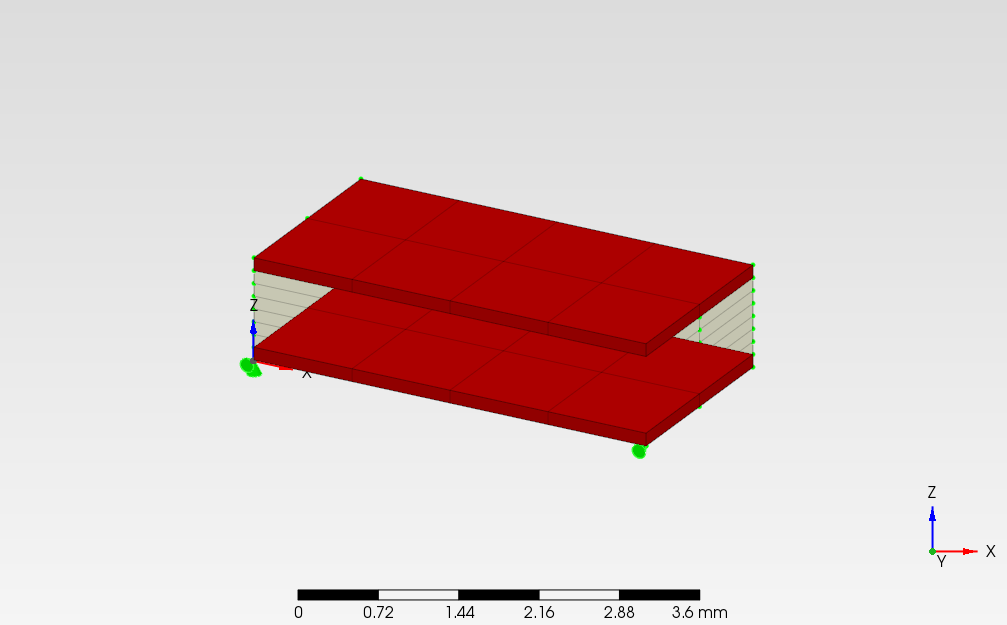
\includegraphics[width=.47\linewidth]{figs/s033_vtk.png}\hfill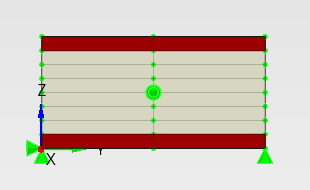
\includegraphics[width=.47\linewidth]{figs/side034_detail.png}
\captionof{figure}{RC1c 既有 VTK：P01 外側兩層的斜視與側視（v3 033--034）。}\label{fig:p01ob}\label{fig:p01side}
\end{center}
\begin{center}
\begin{minipage}{.35\linewidth}\par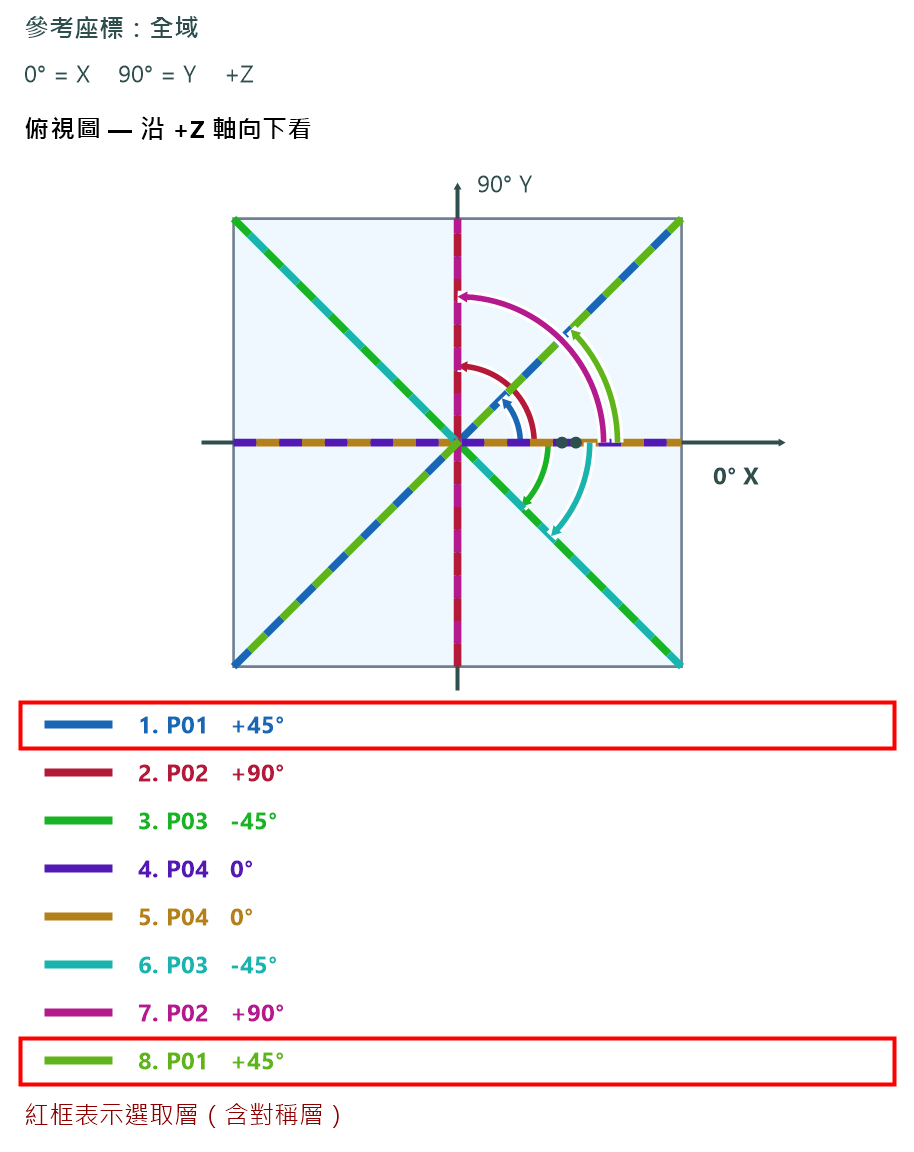
\includegraphics[width=\linewidth]{figs/sym_P01_plan.png}\end{minipage}\hfill
\begin{minipage}{.61\linewidth}\par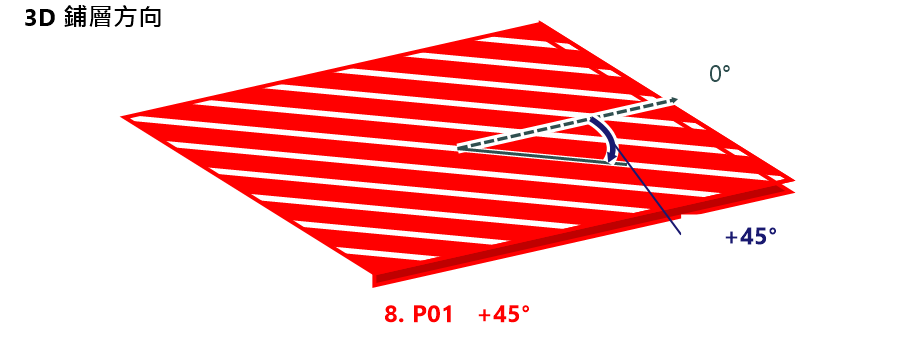
\includegraphics[width=\linewidth]{figs/sym_P01_partner.png}\par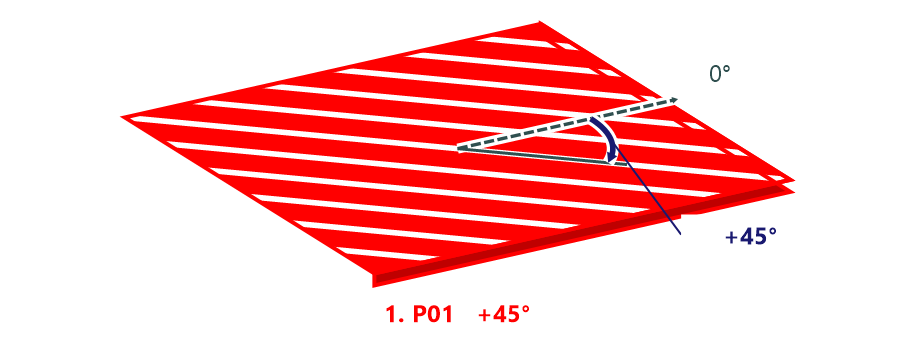
\includegraphics[width=\linewidth]{figs/sym_P01_plate.png}\end{minipage}
\captionof{figure}{RC1g2 選 P01：俯視紅框圈出第 1、8 層；右為上方對稱夥伴與下方原層，兩者均為 $+45^\circ$。}\label{fig:p01native}
\end{center}
以零度箭頭、角度弧與白色纖維線確認方向；紅色選取必須同時對應一對板片。再以 VTK 側視核對實體位置。
由圖\ref{fig:p01ob}的斜視與側視核對：下層 $z=0$--0.125 mm 為元素 1--8，上層 $z=0.875$--1 mm 為元素 57--64，合計 16 個元素。
\note{高亮是選取圖層，可能穿透遮蔽面而可見；不要由穿透紅色誤判增加了其他元素。需同時比對側視位置與第 15 頁實際元素集。}
\page{10\quad 逐層高亮：P02 與 P03}
\textbf{操作 08（v3 035--038）}
依序點 P02、P03，先旋轉看斜視，再切到側視。對照圖\ref{fig:p23native}的 3D／俯視圖、圖\ref{fig:p02}的兩張側視及下表；每列都應高亮 16 個元素。
\begin{center}
\begin{minipage}[t]{.48\linewidth}\centering
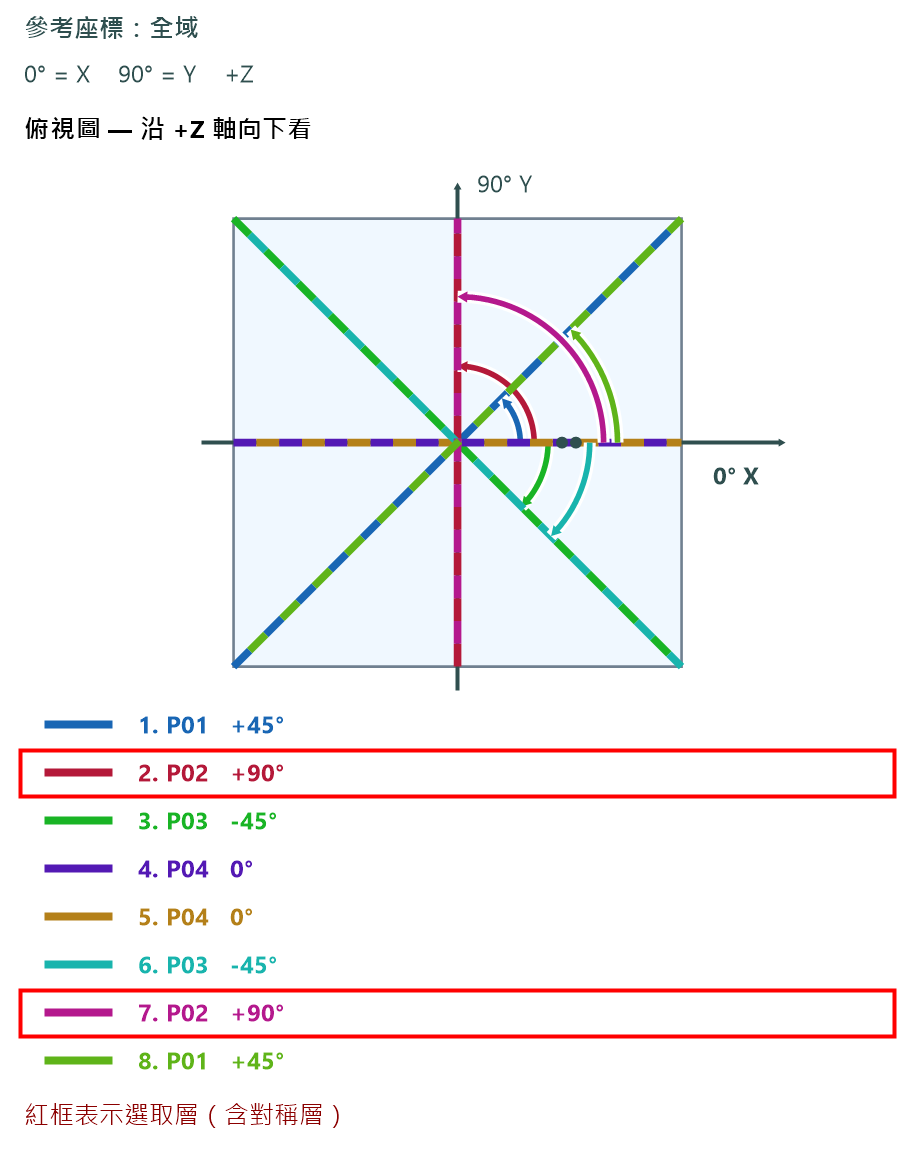
\includegraphics[height=46mm]{figs/sym_P02_plan.png}\par
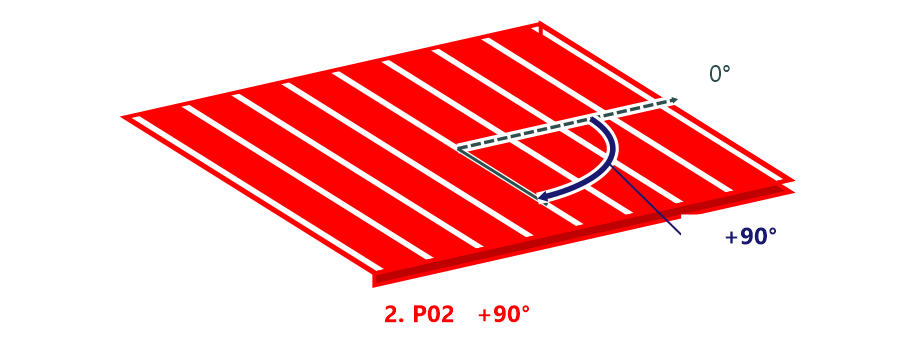
\includegraphics[width=.95\linewidth]{figs/sym_P02_plate.png}
\end{minipage}\hfill
\begin{minipage}[t]{.48\linewidth}\centering
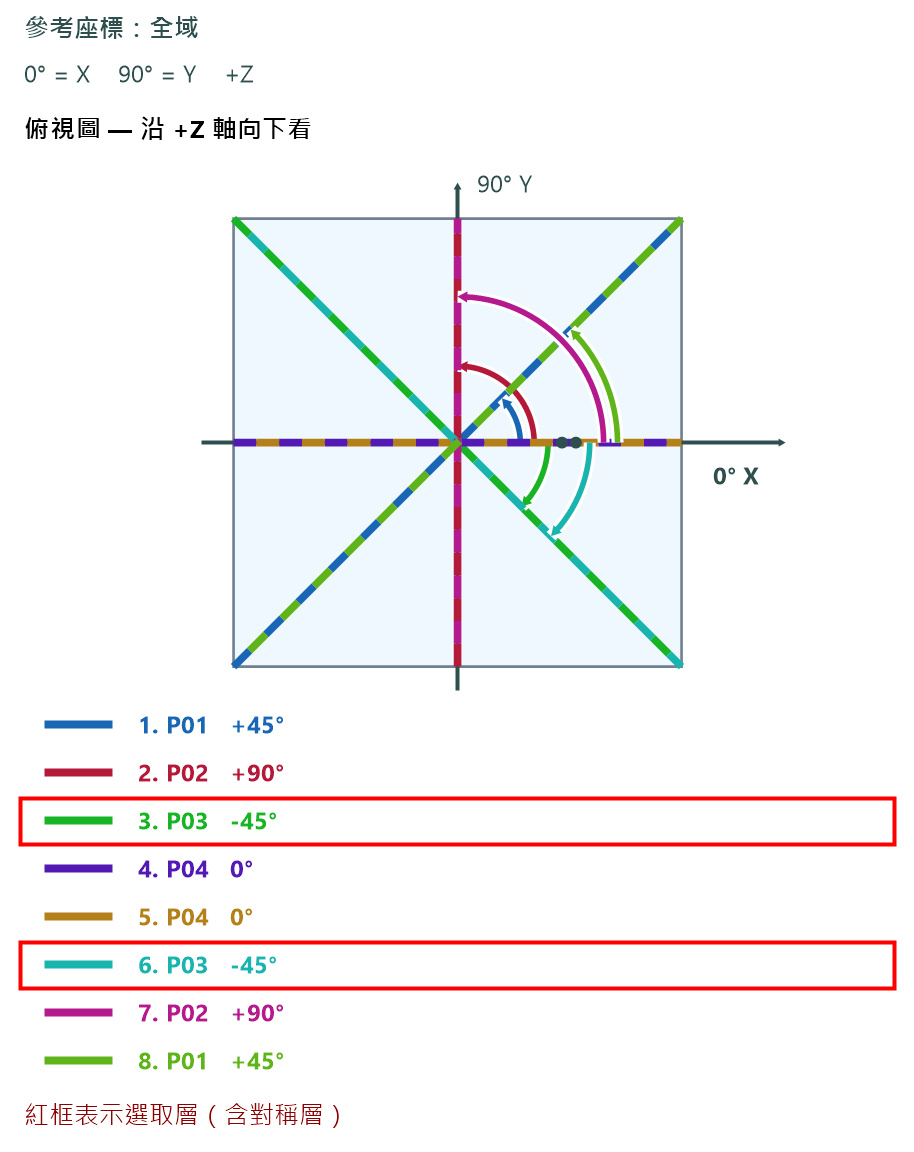
\includegraphics[height=46mm]{figs/sym_P03_plan.png}\par
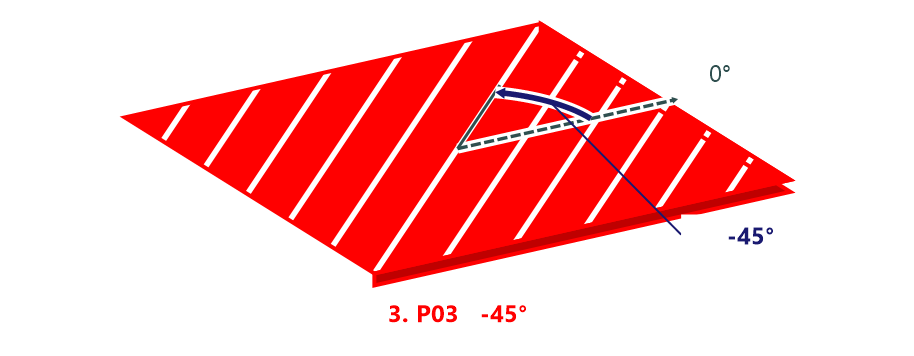
\includegraphics[width=.95\linewidth]{figs/sym_P03_plate.png}
\end{minipage}
\captionof{figure}{RC1g2：左選 P02（$90^\circ$），右選 P03（$-45^\circ$），各裁出所選原層。各俯視紅框同時圈出原層與對稱夥伴，兩者保持相同角度。}\label{fig:p23native}
\end{center}
零度箭頭是基準，角度弧給出正負號；纖維線應分別垂直於零度方向、或呈負 45 度。對稱不反轉角度符號。
\begin{center}
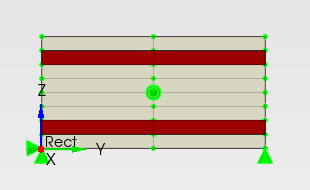
\includegraphics[width=.30\linewidth]{figs/side036_detail.png}\hspace{12mm}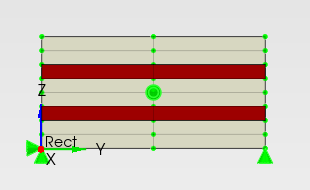
\includegraphics[width=.30\linewidth]{figs/side038_detail.png}
\captionof{figure}{RC1c 既有側視：左 P02（v3 036），右 P03（v3 038）。}\label{fig:p02}\label{fig:p03}
\end{center}
\par\noindent\begin{tabularx}{\linewidth}{@{}lYY@{}}\toprule
輸入列 & 下半層（mm；元素） & 上半對稱層（mm；元素） \\\midrule
P02 & $z=0.125$--0.25；9--16 & $z=0.75$--0.875；49--56 \\
P03 & $z=0.25$--0.375；17--24 & $z=0.625$--0.75；41--48 \\\bottomrule
\end{tabularx}\par
\note{選列時高亮應跟著改變，旋轉後仍貼在正確層。若設定無效，程式會清除前一次的有效高亮；先修正驗證摘要，避免將空白高亮當成繪圖故障。}
\page{11\quad P04、中面與確認儲存}
\textbf{操作 09（v3 039--042）}
選 P04，先檢查斜視、再檢查側視（圖\ref{fig:p04}）。兩個 $0^\circ$ 層相鄰：$z=0.375$--0.5 與 0.5--0.625 mm；元素 25--32 與 33--40，共 16 個。
\begin{center}\par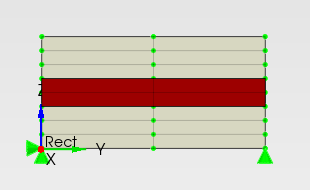
\includegraphics[width=0.40\linewidth]{figs/side040_detail.png}\captionof{figure}{P04 側視局部放大：中央相鄰兩層共同高亮，中面位於兩層之間。來源：v3 步驟 040。}\label{fig:p04}\end{center}
\begin{center}\par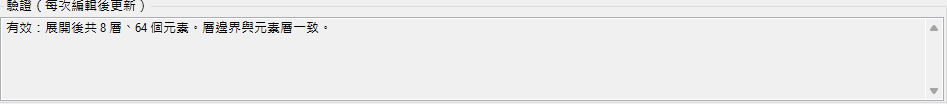
\includegraphics[width=\linewidth]{figs/validation_detail.png}\captionof{figure}{完成後驗證摘要應顯示有效、八層、64 個元素、層邊界與元素層一致。來源：v3 步驟 041 的驗證區。}\label{fig:validation}\end{center}
\begin{center}
\begin{minipage}[c]{.28\linewidth}\par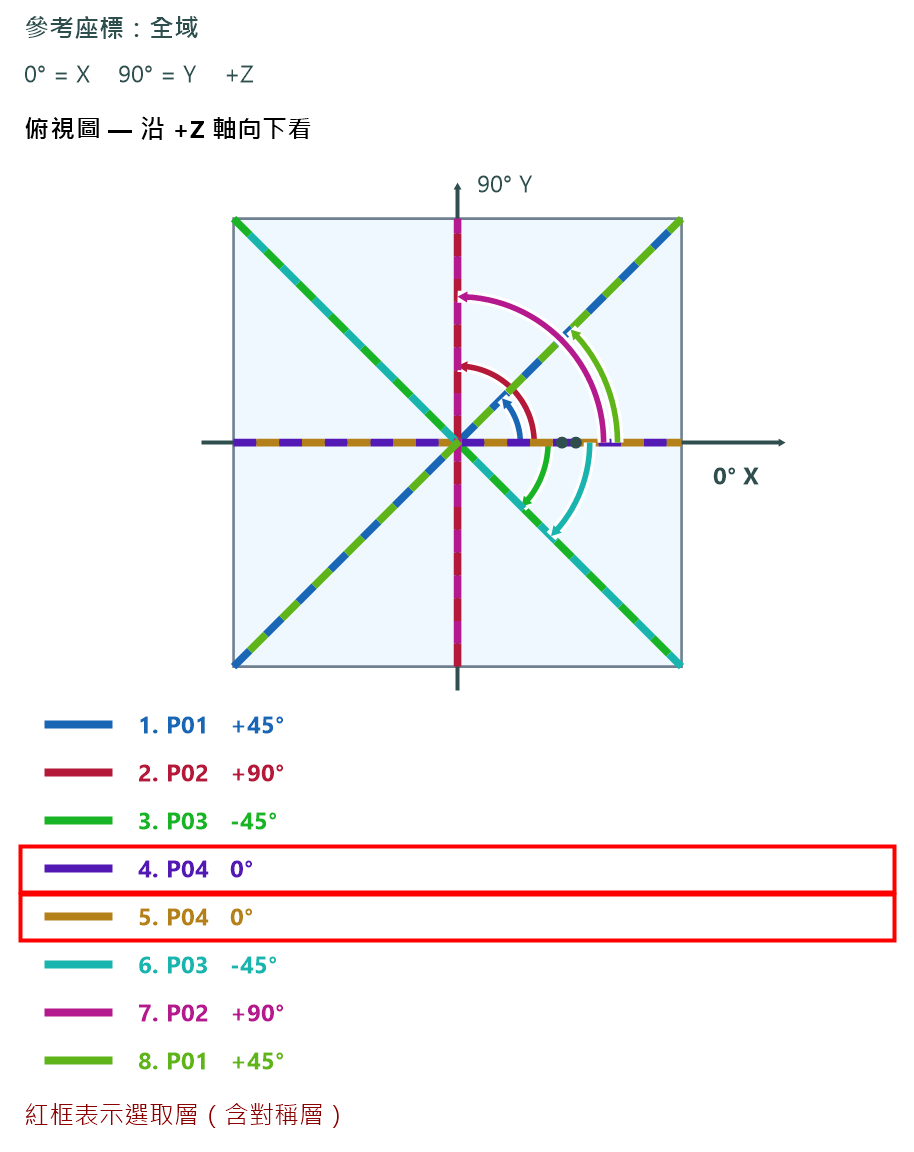
\includegraphics[width=\linewidth]{figs/sym_P04_plan.png}\end{minipage}\hfill
\begin{minipage}[c]{.68\linewidth}\par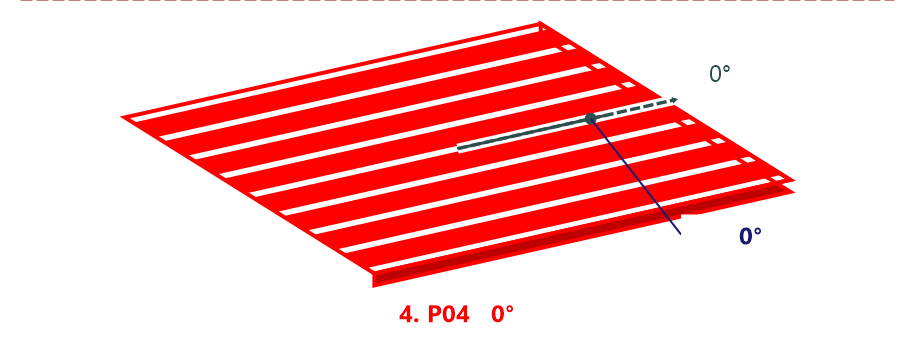
\includegraphics[width=\linewidth]{figs/sym_P04_plate.png}\end{minipage}
\captionof{figure}{RC1g2 選 P04：俯視紅框圈出第 4、5 層；0 度纖維線與虛線箭頭平行。對稱夥伴位於中面另一側，角度相同。}\label{fig:p04native}\end{center}
\subsection*{按確定前逐項完成}
\begin{itemize}
\item 區域為整個試片；Rect／軸 3；對稱是；邊界容差為 1E-06。
\item 四個輸入列的角度為 45、90、−45、0；每列厚度 0.125 mm、元素欄 1、材料 \texttt{IM7\_8552}。
\item 展開八層、總厚度 1 mm；四次高亮各涵蓋兩層，總計覆蓋 64 個不同元素。
\item 圖\ref{fig:validation}的摘要有效，沒有跨層、空層或重複材料指派。
\end{itemize}
按\key{確定}將設定寫入目前模型，再用\key{另存新檔}保留自己的 \texttt{.pmx}。\key{取消}會放棄本次編輯，不更動原有儲存的疊層。
\note{畫面看起來合理還不夠；下一步要看實際匯出的元素集、材料方向與截面連結。}
\page{12\quad 輸入檔核對一：八組元素集}
\textbf{操作 10（v3 043--044、049）}
選\key{模型 → 編輯 CalculiX 關鍵字}，依序查看元素集（Element sets）、材料（Materials）與截面（Sections）群組；再選\key{檔案 → 匯出 → 模型}，於存檔對話框選 \key{CalculiX files (*.inp)}，儲存自己的輸入檔。若介面譯名不同，以 \texttt{ELSET}、\texttt{ORIENTATION}、\texttt{SOLID SECTION} 搜尋定位。
以下逐行引自附帶的 \path{examples/walkthrough_export.inp}，未改寫大小寫或名稱。\texttt{evidence/elsets.inp} 保存同一原文摘錄。
\codefile{elsets}
\textbf{檢核：}八個集合各 8 個元素，合計 64 個，無重複且沒有遺漏。展開索引 01--08 區分兩側的同名 P01--P04；不是只有四個集合。
\note{依序檢查 \texttt{LU\_Walkthrough\_01\_P01} 到 \texttt{LU\_Walkthrough\_08\_P01}，可直接對回第 12--14 頁的高亮位置。若自己的物件名稱不同，前綴名稱會不同，仍須核對層序與集合內容。}
\page{13\quad 輸入檔核對二：方向與正負角度}
\textbf{操作 11（v3 045--046）}
以下為同一範例的全部八組方向原文；沒有用示意數值代替：
\codefile{orientations}
\texttt{1,0,0,0,1,0} 定義基準兩向量 $\mathbf f=+X$、$\mathbf g=+Y$；\texttt{3, 45} 表示繞該局部第三軸旋轉 45 度。八個角度必須為 45、90、−45、0、0、−45、90、45。
另以第\pageref{pg:crosscheck}頁的 3D／俯視圖核對正負號與對稱配對。
\note{匯出旋轉軸欄為局部 3；若 GUI 疊層軸選 1 或 2，匯出會先循環排列基準向量，不能要求關鍵字旋轉軸號必須等於 GUI 軸號。}
\page{13A\quad 用 3D 與俯視核對方向原文}\label{pg:crosscheck}
先讀上一頁的八組 \texttt{*ORIENTATION}，再回到 RC1g2 選 P01--P04。四個所選原層在下方並排；相同角度的對稱夥伴不改符號。
\begin{center}
\begin{tabular}{@{}cccc@{}}
\begin{minipage}{.23\linewidth}\centering P01 / $+45^\circ$\par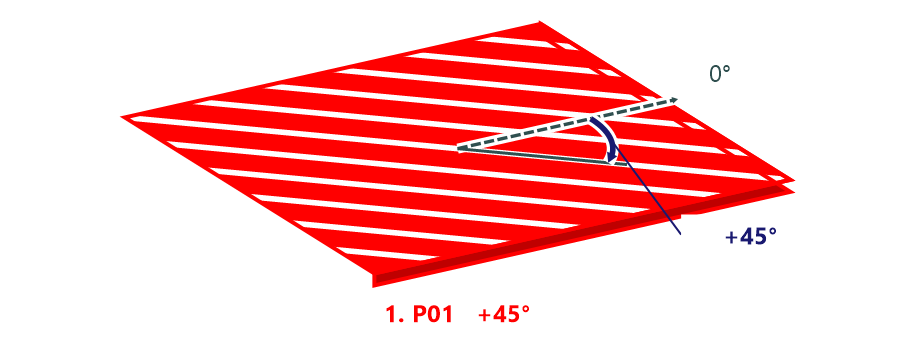
\includegraphics[width=\linewidth]{figs/sym_P01_plate.png}\end{minipage}&
\begin{minipage}{.23\linewidth}\centering P02 / $90^\circ$\par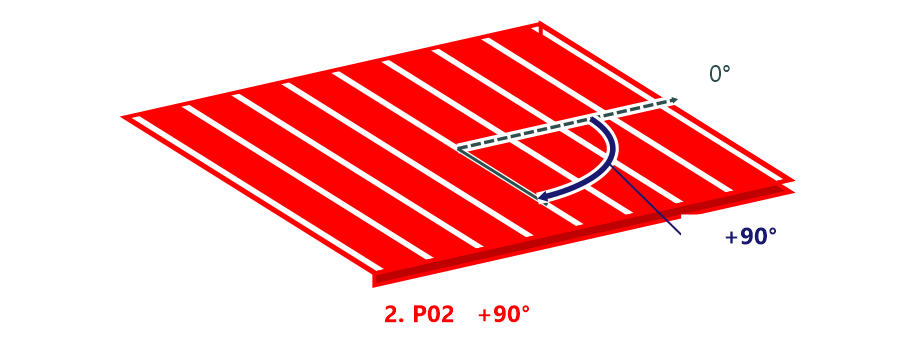
\includegraphics[width=\linewidth]{figs/sym_P02_plate.png}\end{minipage}&
\begin{minipage}{.23\linewidth}\centering P03 / $-45^\circ$\par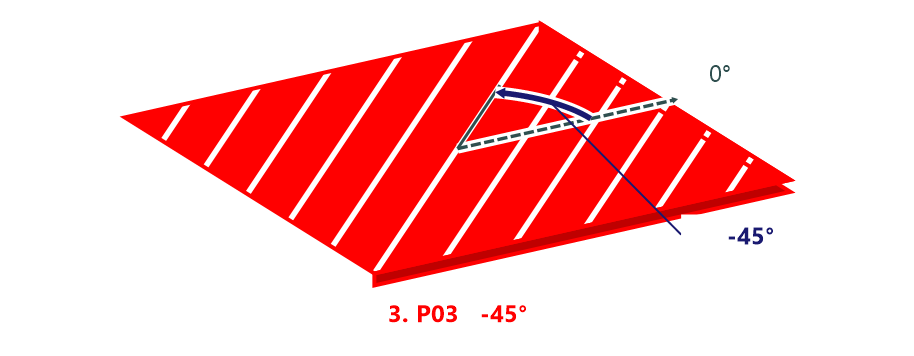
\includegraphics[width=\linewidth]{figs/sym_P03_plate.png}\end{minipage}&
\begin{minipage}{.23\linewidth}\centering P04 / $0^\circ$\par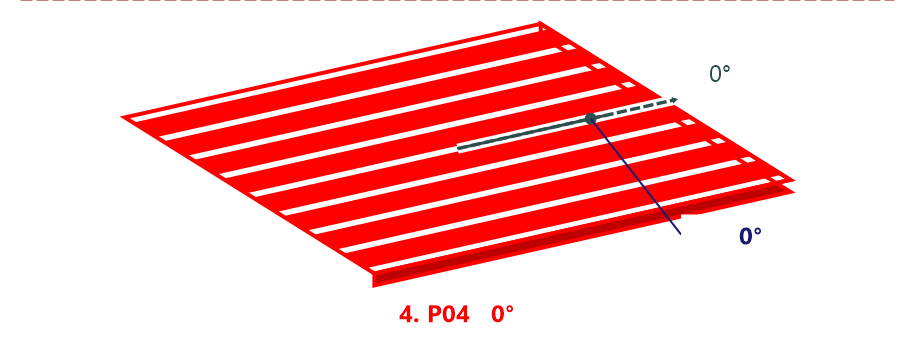
\includegraphics[width=\linewidth]{figs/sym_P04_plate.png}\end{minipage}
\end{tabular}
\captionof{figure}{RC1g2 四次選取的 3D 原層裁切；各自的角度弧從同一 $0^\circ$ 箭頭起算。}\label{fig:crossplates}
\end{center}
\begin{center}\par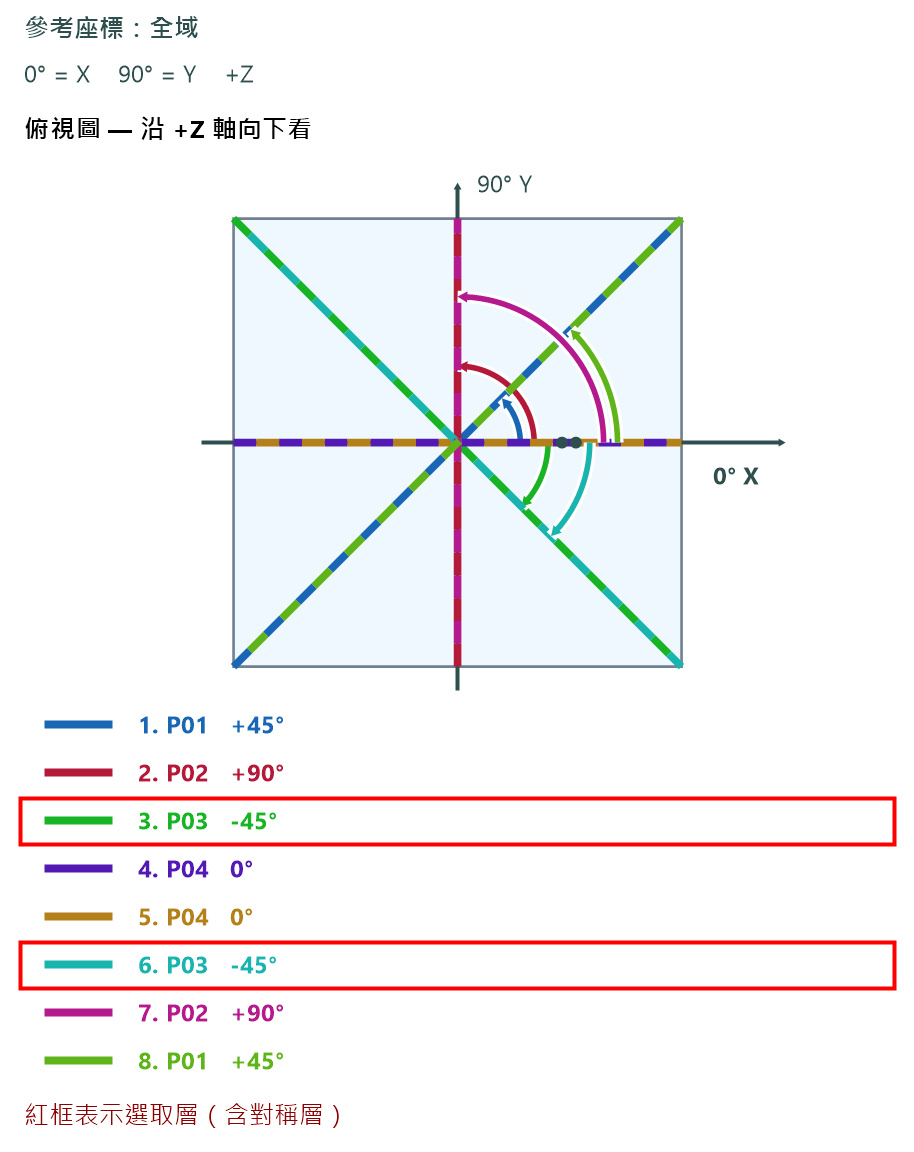
\includegraphics[height=105mm]{figs/sym_P03_plan.png}
\captionof{figure}{RC1g2 對稱例俯視圖：$+45/-45$ 成 X，$0/90$ 為水平與垂直；此圖選 P03，紅框為第 3、6 層。}\label{fig:crossplan}\end{center}
\begin{enumerate}
\item 核對參考座標與疊層軸。本例 $0^\circ=+X$、$90^\circ=+Y$；俯視正角度逆時針。
\item 核對輸入列、3D 角度標值和纖維線，再比對八組輸出的角度順序。第 3、6 層均為 $-45$，不能變成 $+45$。
\item 用紅框及紅色板片確認所選層與對稱夥伴，再以元素集、側視與截面連結確認作用位置。
\end{enumerate}
\note{3D 視覺、俯視圖、原文關鍵字三者應一致；螢幕透視角不是材料角度。若不一致，回到可編輯模型修正後重新匯出。}

\page{14\quad 輸入檔核對三：截面連結}
\textbf{操作 12（v3 047--048）}
以下八行原文把元素集、材料與方向逐一連結。為適應紙寬，長行自動折行；\texttt{evidence/sections.inp} 與原始輸出仍各為一個完整關鍵字行。
\codefile{sections}
\subsection*{逐行核對三個欄位}
\begin{enumerate}
\item \texttt{ELSET=} 的索引與第 15 頁集合一致。
\item \texttt{MATERIAL=IM7\_8552} 指向模型中的真實層材料。
\item \texttt{ORIENTATION=} 的索引和 P 名稱與該集合一致，例如第 03 層必須指到 \texttt{OR\_Walkthrough\_03\_P03}，角度為 $-45^\circ$。
\end{enumerate}
\note{實體層厚由節點座標與元素集合表示；這些 \texttt{*SOLID SECTION} 行不另填一個殼厚度。只看到方向關鍵字存在，仍不足以證明方向已正確套用到每一層。}
開啟自己的 \texttt{.inp} 與附帶範例比對時，名稱、數值及層序應符合自己的設計。若預覽報錯，先修復模型；不要用手改輸出檔代替修正可編輯的疊層。
\page{15\quad 執行分析並核對結果}
\textbf{操作 13（v3 050--053）}
\begin{enumerate}
\item 在求解器設定確認使用 RC1g2 隨附的 \texttt{Solver/ccx\_fat.exe}（v1.1b），矩陣解法 Spooles；分析工作 CPU 數設為 1，工作目錄用自己的可寫入資料夾。
\item 在\key{分析（Analyses）}樹建立／編輯工作，命名 \texttt{Walkthrough}，確認使用目前模型，再右鍵執行。保留起點原有的靜態步與邊界條件，不額外施加新載重。
\item 等待完成，先確認求解器正常結束、沒有 \texttt{*ERROR}。開啟輸出的 \texttt{Walkthrough.frd}，選 DISP／位移分量查看結果（圖\ref{fig:result}）。
\end{enumerate}
\shot{s052_vtk.png}{0.90}{v3 步驟 052 的原生 VTK 位移結果（RC1c 來源）；保留圖例與變形倍率，未包含工作站標題列或日誌。}{fig:result}
本例 $L_x=4$ mm、$A=2\times1=2$ mm$^2$、施加位移 $u_x=0.0004$ mm，因此 $\epsilon_x=10^{-4}$。\texttt{Walkthrough.dat} 的 X1 總反力為 12.10015 N，故
\[E_x^{\mathrm{app}}=\frac{RF_x}{A\epsilon_x}=\frac{12.10015}{2\times10^{-4}}=60500.75\ \mathrm{MPa}.\]
\note{這是有限自由邊試片的表觀值，不是無限板 CLT 模數。相同層材料的週期膜單元 CLT 基準約 64387.645 MPa；邊界條件不同，不可混當同一驗收值。RC1f/v1.1b 的既有回歸也給出 60500.75 MPa，本文件未另做新求解。}
\page{16\quad 常見錯誤與完成檢查}
\par\noindent\begin{tabularx}{\linewidth}{@{}P{34mm}YY@{}}\toprule
現象／錯誤 & 原因 & 處理與通過條件 \\\midrule
總厚度不符 & 只輸入半疊層；或完整八層又啟用對稱。 & 以展開後厚度合計比對區域投影厚度。本例須八層、1 mm。 \\
總厚度對但元素跨層 & 層界切穿元素；可能連中間節點也跨界。 & 修正層厚或網格。兩個 0.5 mm 元素層不能直接當四個 0.25 mm 層。 \\
「元素」欄錯誤 & 把 8 個元素總數或 ID 填入。 & 本例每 0.125 mm 層是一帶，填 1；選填欄留空不代表免除跨層檢查。 \\
空層或高亮全空 & 區域、軸或層厚錯；無效設定會清除舊高亮。 & 先讀摘要，再核對區域實體元素與投影方向。 \\
角度正負看似相反 & 用畫面朝向猜測局部軸；或參考座標系已旋轉。 & 以第\pageref{pg:angles}頁的零度箭頭、角度弧與俯視圖核對，再查方向原文。 \\
重疊指派 & 多個啟用疊層或一般材料截面覆蓋同一元素。 & 停用重複物件；複製的疊層也會獨立生效。 \\
材料／座標系遺失 & 依賴物件被刪除、停用或無效。 & 重新指定有效材料、直角座標系及區域；不要只改顯示名稱。 \\
重新匯入後無疊層樹 & \texttt{.inp} 只存展開後求解內容。 & 用原 \texttt{.pmx} 繼續編輯。舊版也不保證能讀取含新疊層的 \texttt{.pmx}。 \\\bottomrule
\end{tabularx}\par
\subsection*{交給老師或 AI 複核時附上}
\begin{itemize}
\item 可編輯 \texttt{.pmx}、實際匯出 \texttt{.inp}、求解器版本與正常結束紀錄。
\item 區域元素數、參考座標系、疊層軸、對稱值、逐層材料／厚度／角度／帶數。
\item 展開後層序、各層元素集、3D 纖維線／俯視 X 與逐層高亮／側視證據。
\item 若比較數值，說明載重、邊界條件、單位與反力換算式。
\end{itemize}
\note{驗證摘要通過是必要條件；它不代替對材料參數、設計合理性與邊界條件的工程判斷。}
\page{17\quad 繁體中文術語對照}
本文操作與術語以 RC1g2 隨附 zh-TW 字庫為準。既有 RC1c 影格中的舊譯保留原貌，請依本表對照 RC1g2；材料名與求解器關鍵字維持原名。
\par\noindent\begin{tabularx}{\linewidth}{@{}P{38mm}P{44mm}Y@{}}\toprule
英文／識別詞 & 本文用語 & 意義／舊畫面對照 \\\midrule
3D ply orientation & 3D 鋪層方向 & RC1g2 編輯器的分離板片預覽；以零度箭頭、角度弧及纖維線讀方向。 \\
Plan view & 俯視圖 & 沿正疊層軸向下看；彩線疊合各層方向，紅框為選取層及對稱層。 \\
Composite layup & 複材疊層 & 逐層的材料、厚度與角度定義；舊處可能稱複合材料疊層。 \\
Ply & 單層／層片 & P01 等輸入列；選對稱後可對應兩個實體層。 \\
Delamination & 分層 & 層間分離的損傷現象；不是建立疊層表格的同義詞。 \\
Crack & 裂紋 & 舊譯可能為裂縫；本教學統一稱裂紋。 \\
Load & 載重 & 舊譯可能為負載或載荷；本教學統一稱載重。 \\
Amplitude & 幅值曲線 & 載重等隨時間變化的倍率；不可與角度混淆。 \\
FATCZM & 疲勞內聚力模型（FATCZM） & RC1g2 UI 使用此名稱；其材料與界面需另外設定。 \\
Region type & 區域類型 & 零件名稱、元素集名稱或選取範圍。 \\
Stacking axis & 疊層軸 & 厚度正方向；有些旁白稱堆疊軸，兩者同義。 \\
Reference CSYS & 參考座標系 & UI 常為座標系統；Global 或直角座標系。 \\
Boundary tolerance & 邊界容差 & 相對於完整展開厚度的容差。 \\
Elements & 厚度網格帶數 & 此疊層表格中的「元素」欄，非元素 ID 清單。 \\
Orientation & 材料方向 & \texttt{*ORIENTATION}；定義層片的纖維方向。 \\
Solid section & 實體截面 & 舊譯可見實體斷面；連結元素集、材料與方向。 \\
CalculiX & CalculiX 求解器 & 舊關鍵字編輯器可能誤譯成「微積分」；它是程式名。 \\\bottomrule
\end{tabularx}\par
\note{分層（損傷）與疊層（材料排列）不同。本例為沒有 FATCZM 界面的連續實體疊層，不能由其完成求解推論已模擬分層或疲勞裂紋成長。}
\page{附錄 A\quad 版本、檔案與可重建來源}
\subsection*{版本與證據範圍}
\par\noindent\begin{tabularx}{\linewidth}{@{}lY@{}}\toprule
項目 & 本教學使用的來源 \\\midrule
目標發行 & PrePoMax-RCM RC1g2，隨附 ccx\_fat v1.1b。新增圖由 RC1g2 擷取；60500.75 MPa 為既有 RC1f/v1.1b 結果，本次未重跑求解。 \\
影片內容 & \texttt{narration\_script\_zh-TW\_v3.md}，53 步；031 明確修訂為對稱可選、預設否。 \\
截圖 & RC1g2 原生 3D／俯視面板：兩層各一次、對稱例四次選取；既有表單／VTK 為 RC1c，未改標為 RC1g2。 \\
技術與人工檢查 & \texttt{COMPOSITE\_LAYUP.md}、\texttt{M2b\_HUMAN\_CHECK\_zh-TW.md}。後者為內部兩層檢查，其網格與本教學不同；本教學的可重做帶數以所附起點為準。 \\
樣式依據 & RC1f \texttt{快速入門\_zh-TW.pdf}：A4、深藍／青綠、編號學習順序、頁碼與 Isisam 署名；本文改以 XeLaTeX、Noto CJK TC 編譯。 \\\bottomrule
\end{tabularx}\par
\subsection*{來源包與相對位置}
解壓來源 ZIP 後，以 \texttt{tutorial\_layup/} 為主目錄。\texttt{main.tex} 是正文；\texttt{figs/} 是正文圖像；\texttt{examples/} 包含起點、完成的求解輸入與既有結果；不附 PMX，請依本文建立疊層後自行儲存；\texttt{evidence/} 包含技術慣例、v3 旁白及逐字關鍵字摘錄。
\texttt{README.md} 說明重建方式；\texttt{SOURCE\_MANIFEST.json} 記錄來源檔案雜湊。所有編譯輸入採相對路徑，不需原製作工作站或網路磁碟。
\subsection*{來源與版本核對}
\texttt{evidence/EXTERNAL\_EVIDENCE.md} 記錄原生影格來源、RC1f 求解器校驗值及結果依據。原始內部執行報告及建置輔助腳本不隨對外來源包提供；技術依據為所附 \texttt{COMPOSITE\_LAYUP.md}。
\subsection*{交付檔案}
\cjkpath{08_疊層設定教學_v2_3D.pdf}\par
\cjkpath{08_疊層設定教學_v2_3D_src.zip}\par
請將 PDF 與來源 ZIP 一起保存。讀者可在自己的可寫入目錄解壓並重建，不需對應製作者的磁碟代號。
\page{附錄 B\quad v3 逐段對照與重建}
\par\noindent\begin{tabularx}{\linewidth}{@{}lYl@{}}\toprule
v3 步驟 & 本文涵蓋內容 & 頁次 \\\midrule
001--002 & 無疊層副本、64 元素、八帶、3D／mm & 4--5 \\
003--005 & Walkthrough 名稱、區域類型與零件 & 5 \\
006--007 & Rect、第三軸、Z 正向；補充容差 & 2、6 \\
008--012 & P01 材料、0.125 mm、45 度、1 帶 & 7 \\
013--018 & P02 新增、材料、厚度、90 度、1 帶 & 8 \\
019--024 & P03 新增、材料、厚度、−45 度、1 帶 & 8 \\
025--030 & P04 新增、材料、厚度、0 度、1 帶 & 8 \\
031--032 & 可選對稱、預設否、八層展開與中面 & 9--11 \\
033--034 & P01 斜視與側視、兩端 16 元素 & 12 \\
035--036 & P02 斜視／側視與元素位置 & 13 \\
037--038 & P03 斜視／側視與元素位置 & 13 \\
039--040 & P04 中央兩層與側視 & 14 \\
041--042 & 八層／64 元素檢核、確定與儲存 & 14 \\
043--044 & 全八組 ELSET 原文 & 15 \\
045--046 & 全八組 ORIENTATION 原文 & 16--17 \\
047--048 & 全八組 SOLID SECTION 原文 & 18 \\
049--053 & 匯出、單 CPU 求解、反力、FRD 與檔案 & 15、19 \\
補充 & 複製、反轉、兩層不對稱、錯誤及術語 & 9--10、20--21 \\\bottomrule
\end{tabularx}\par
\subsection*{XeLaTeX 重建（WSL Ubuntu-24.04）}
將目錄置於可寫入的 WSL 路徑，在該目錄執行兩次：
\begin{Verbatim}[fontsize=\small,frame=single]
xelatex -interaction=nonstopmode -halt-on-error main.tex
xelatex -interaction=nonstopmode -halt-on-error main.tex
\end{Verbatim}
字型：\texttt{Noto Serif CJK TC}、\texttt{Noto Sans CJK TC}；西文字型 TeX Gyre Pagella／Heros，等寬 DejaVu Sans Mono。無需網路資源即可重編。套件與相對路徑檢查方式見 README。
\note{本文件所有畫面僅為 PrePoMax 原生表單與視圖。RC1g2 新圖僅裁切面板，保留零度箭頭、角度弧、纖維線與選取標示；各圖說分別列出來源版本。裁切圖保留原始欄位；文字說明、原始 \texttt{.inp} 與版本證據均隨來源包附上，方便逐項複核。}
\end{document}
